% !TEX encoding = UTF-8 Unicode
% !TEX program = pdflatex
\documentclass[12pt,a4paper]{report}
\usepackage{cmap}
\usepackage[utf8]{inputenc}
\usepackage[T5]{fontenc}
\usepackage[utf8]{vietnam}
\usepackage{./StylelatexformTBU(datdatcre)/tbu_report}
\usetikzlibrary{shapes.geometric, arrows.meta, positioning, calc, fit, chains}

% Set line spacing for academic report
\setstretch{1.3}

% ==============================================================================
% CẤU HÌNH THÔNG TIN BÁO CÁO BÀI TẬP LỚN
% ==============================================================================
\ministry{BỘ GIÁO DỤC VÀ ĐÀO TẠO}
\university{TRƯỜNG ĐẠI HỌC TÂY BẮC}
\faculty{KHOA CÔNG NGHỆ THÔNG TIN}
\reporttype{BÁO CÁO BÀI TẬP LỚN MÔN HỌC}
\title{QUẢN LÝ QUẦN CHÚNG ƯU TÚ PHỤC VỤ KẾT NẠP ĐẢNG}
\courseclass{K64 ĐẠI HỌC CNTT}
\groupnumber{Nhóm 02}
\advisor{ThS. Đặng Thị Vân Chi}
\location{SƠN LA}
\reportdate{THÁNG 08/2026}
\logopath{./StylelatexformTBU(datdatcre)/tbu_logo.png}

% Danh sách Sinh viên thực hiện (4 thành viên)
\addstudent[NT]{Lò Mạnh Đạt}
\addstudent{Nguyễn Huy Hoàng}
\addstudent{Tòng Lưu Anh Tú}
\addstudent{Phạm Thị Thanh Hảo}

\begin{document}
\pagenumbering{gobble}

% ==============================================================================
% 1. TRANG BÌA NGOÀI VÀ TRANG BÌA PHỤ
% ==============================================================================
\makeoutercover
\makeinnercover

% ==============================================================================
% 2. LỜI CẢM ƠN
% ==============================================================================
\begin{acknowledgements}
  Chúng em xin gửi lời cảm ơn chân thành và sâu sắc nhất đến Cô ThS. Đặng Thị Vân Chi đã tận tình giảng dạy, truyền đạt những kiến thức chuyên môn quý báu và định hướng cho nhóm trong suốt quá trình học tập và thực hiện bài tập lớn môn học này.

  Dù nhóm đã rất cố gắng trong việc hoàn thành bài tập lớn "Quản lý Quần chúng Ưu tú Phục vụ Kết nạp Đảng", bài báo cáo vẫn khó tránh khỏi những hạn chế và thiếu sót. Nhóm kính mong nhận được sự đóng góp ý kiến từ Cô và các bạn để sản phẩm bài tập lớn được hoàn thiện và nâng cao tính ứng dụng thực tiễn hơn trong tương lai.
\end{acknowledgements}

% ==============================================================================
% 3. MỤC LỤC VÀ DANH MỤC TỪ VIẾT TẮT, DANH MỤC HÌNH ẢNH, DANH MỤC BẢNG BIỂU
% ==============================================================================
\makecontentlists

\cleardoublepage
\section*{BẢNG PHÂN CÔNG NHIỆM VỤ THỰC HIỆN DỰ ÁN}
\vspace{0.5em}
{\setstretch{1.3}\fontsize{10pt}{13pt}\selectfont
  \begin{xltabular}{\linewidth}{|c|l|c|X|}
    \hline
    \textbf{STT} & \textbf{Họ và Tên} & \textbf{MSSV} & \textbf{Phân công Nhiệm vụ} \\ \hline
    \endfirsthead
    \hline
    \textbf{STT} & \textbf{Họ và Tên} & \textbf{MSSV} & \textbf{Phân công Nhiệm vụ} \\ \hline
    \endhead
    \hline
    \endfoot
    1 & LÒ MẠNH ĐẠT        & 2023A0861 & Backend PHP, Database, Agent AI, Báo cáo \\ \hline
    2 & NGUYỄN HUY HOÀNG   & 2023A0875 & Frontend Python API, Edge AI             \\ \hline
    3 & TÒNG LƯU ANH TÚ    & 2023A0937 & Báo cáo CSS/JS, UI/UX, Edge AI           \\ \hline
    4 & PHẠM THỊ THANH HẢO & 2023A0869 & Database, Báo cáo                        \\ \hline
  \end{xltabular}
  \label{tab:phan_cong_nhom_readme}}
\cleardoublepage

\begin{abbreviations}
  AI & Artificial Intelligence (Trí tuệ Nhân tạo) \\ \hline
  API & Application Programming Interface (Giao diện Lập trình Ứng dụng) \\ \hline
  BEM & Block Element Modifier (Tiêu chuẩn Đặt tên Class CSS) \\ \hline
  CCCD & Căn cước công dân \\ \hline
  CSDL & Cơ sở dữ liệu \\ \hline
  DOM & Document Object Model (Mô hình Đối tượng Tài liệu Web) \\ \hline
  DOI & Digital Object Identifier (Mã Định danh Đối tượng Số) \\ \hline
  ERD & Entity Relationship Diagram (Sơ đồ Quan hệ Thực thể) \\ \hline
  JS & JavaScript \\ \hline
  JSON & JavaScript Object Notation (Định dạng Trao đổi Dữ liệu Kịch bản) \\ \hline
  MVC & Model - View - Controller (Mô hình Kiến trúc Phần mềm) \\ \hline
  OCR & Optical Character Recognition (Nhận dạng Ký tự Quang học) \\ \hline
  PDO & PHP Data Objects (Lớp Kết nối Cơ sở Dữ liệu Chuẩn trong PHP) \\ \hline
  PDF & Portable Document Format (Định dạng Tài liệu Di động) \\ \hline
  PWA & Progressive Web Application (Ứng dụng Web Lũy tiến) \\ \hline
  RBAC & Role-Based Access Control (Kiểm soát Truy cập Dựa trên Vai trò) \\ \hline
  RSS & Really Simple Syndication (Dịch vụ Cung cấp Thông tin Tóm tắt) \\ \hline
  TBU & Tay Bac University (Trường Đại học Tây Bắc) \\ \hline
  UI/UX & User Interface / User Experience (Giao diện \& Trải nghiệm Người dùng) \\ \hline
  WASM & WebAssembly (Định dạng Mã nhị phân Thực thi trên Trình duyệt) \\
\end{abbreviations}

\cleardoublepage
\renewcommand{\listfigurename}{DANH MỤC HÌNH ẢNH}
\listoffigures
\cleardoublepage

\cleardoublepage
\renewcommand{\listtablename}{DANH MỤC BẢNG BIỂU}
\listoftables
\cleardoublepage

\cleardoublepage
% ==============================================================================
% TẮT NGẮT TRANG TRONG PHẦN NỘI DUNG CHÍNH (NỐI LIỀN NỘI DUNG BẰNG VSPACE)
% ==============================================================================
\makeatletter
\let\oldcleardoublepage\cleardoublepage
\let\oldclearpage\clearpage
\renewcommand{\cleardoublepage}{\par\vspace{1.5em}}
\renewcommand{\clearpage}{\par\vspace{1.5em}}
\makeatother

% ==============================================================================
% 4. NỘI DUNG CHÍNH CỦA BÁO CÁO (ĐÁNH SỐ TRANG BẮT ĐẦU TỪ PHẦN MỞ ĐẦU)
% ==============================================================================
\pagenumbering{arabic}
\setcounter{page}{1}

\section*{I. MỞ ĐẦU VÀ TÍNH CẤP THIẾT CỦA ĐỀ TÀI}
\addcontentsline{toc}{section}{I. MỞ ĐẦU VÀ TÍNH CẤP THIẾT CỦA ĐỀ TÀI}

Trong bối cảnh đẩy mạnh chuyển đổi số quốc gia và hiện đại hóa công tác hành chính trong các cơ quan, tổ chức chính trị -- xã hội, việc ứng dụng công nghệ thông tin vào công tác Đảng vụ tại các trường đại học đóng vai trò quan trọng nhằm chuẩn hóa quy trình, nâng cao tính chính xác và hỗ trợ an toàn thông tin. Phần mở đầu trình bày tổng quan bối cảnh thực tiễn, phân tích các hạn chế của phương thức thủ công, xác lập mục tiêu nghiên cứu và định hình phương pháp luận phát triển của đề tài.

\subsection*{1.1 Bối cảnh thực tiễn và tính cấp thiết}
\addcontentsline{toc}{subsection}{1.1 Bối cảnh thực tiễn và tính cấp thiết}
Công tác quản lý, bồi dưỡng và kết nạp Đảng viên tại các cơ sở giáo dục đại học là quy trình nghiệp vụ hành chính có tính bảo mật cao, nhiều giai đoạn thẩm định và tuân thủ nghiêm ngặt các quy định của Điều lệ Đảng cùng Hướng dẫn số 01-HD/TW ngày 28/9/2021 của Ban Tổ chức Trung ương. Quy trình kéo dài từ khâu tiếp nhận hồ sơ cảm tình Đảng, theo dõi rèn luyện, phân công Đảng viên hướng dẫn, đến thẩm định 5 mẫu tài liệu minh chứng đầu vào (Bản tự nhận xét, Giấy chứng nhận học lớp Đảng, Sơ yếu lý lịch, Phiếu đánh giá đoàn viên và Giấy khen).

Trong bối cảnh chuyển đổi số giáo dục và xây dựng chính phủ điện tử, phương thức quản lý hồ sơ thủ công bộc lộ nhiều điểm nghẽn về thời gian xử lý, tính toàn vẹn dữ liệu và tính minh bạch \cite{nusa2020iop, nofrianda2022jictas}. Tại Trường Đại học Tây Bắc (TBU), việc quản lý tập trung danh sách quần chúng ưu tú đòi hỏi một hệ thống thông tin chuyên dụng, phân quyền chặt chẽ theo mô hình RBAC và tích hợp các giải pháp trí tuệ nhân tạo biên (Edge AI) nhằm hỗ trợ tự động hóa khâu xử lý tài liệu minh chứng hành chính.

\subsection*{1.2 Phân tích các hạn chế của quy trình quản lý thủ công}
\addcontentsline{toc}{subsection}{1.2 Phân tích các hạn chế của quy trình quản lý thủ công}
Từ thực tế triển khai công tác Đảng vụ tại cơ sở, quy trình quản lý truyền thống dựa trên giấy tờ và các bảng tính phân tán gặp phải 6 hạn chế kỹ thuật cốt lõi:
\begin{enumerate}[label=\arabic*.]
  \item Nguy cơ thất lạc và suy giảm chất lượng vật lý: Khối lượng hồ sơ giấy lớn qua nhiều năm theo dõi dễ hư hỏng, thất lạc trong quá trình lưu trữ và luân chuyển giữa các cấp Chi bộ.
  \item Độ trễ và sai sót trong đối soát thủ công: Cán bộ Đảng vụ phải kiểm tra thủ công từng trường thông tin (Họ tên, Ngày sinh, Số quyết định) trên bản in, tiêu tốn trung bình 45--60 phút/bộ hồ sơ và dễ bỏ sót các trường thông tin khuyết.
  \item Thiếu cơ chế theo dõi tiến trình thời gian thực: Quần chúng ưu tú không thể tra cứu trực tuyến trạng thái xử lý hồ sơ trong quy trình xét duyệt 5 bước.
  \item Bất đồng bộ dữ liệu tổng hợp: Thu thập dữ liệu từ các tệp Excel phân tán dẫn đến tình trạng trùng lặp bản ghi, sai lệch định dạng ngày tháng và không thống nhất danh mục Chi bộ.
  \item Lỗi cấu trúc tiêu đề khi nhập liệu: Tệp dữ liệu đầu vào từ các lớp có tiêu đề cột không đồng nhất hoặc bị khuyết ô tiêu đề, gây sai lệch nghiêm trọng khi ánh xạ vào cơ sở dữ liệu.
  \item Chi phí in ấn và chu kỳ hiệu chỉnh kéo dài: Mỗi thay đổi nhỏ về thông tin cá nhân đều yêu cầu in ấn lại toàn bộ bộ hồ sơ, làm gia tăng chi phí và kéo dài tiến độ phê duyệt.
\end{enumerate}

\subsection*{1.3 Mục tiêu nghiên cứu và chỉ số định lượng}
\addcontentsline{toc}{subsection}{1.3 Mục tiêu nghiên cứu và chỉ số định lượng}
Nhằm khắc phục triệt để các hạn chế kỹ thuật nêu trên, đề tài xác lập mục tiêu nghiên cứu tổng quát cùng các chỉ tiêu đo lường kỹ thuật trong phạm vi thử nghiệm:
\begin{itemize}[label=--,leftmargin=*]
  \item Mục tiêu tổng quát: Xây dựng hệ thống thông tin Web phân tầng bảo mật và hiệu năng cao, số hóa toàn diện quy trình quản lý quần chúng ưu tú từ khâu đăng ký, thẩm định hồ sơ, theo dõi rèn luyện đến kết xuất 8 biểu mẫu kết nạp Đảng chuẩn thể thức hành chính.
  \item Chỉ số kỹ thuật định lượng (Mục tiêu thiết kế):
        \begin{itemize}[label=--,leftmargin=*]
          \item Phân hệ Edge AI OCR: Nhận dạng ký tự quang học trực tiếp tại Client qua \texttt{Tesseract.js} (WASM) với thời gian xử lý $< 2.5$ giây/trang, độ chính xác trích xuất CCCD $\ge 95$\% \cite{singh2023edgeai, passarotto2024edge}.
          \item Phân hệ Multi-Agent AI Inspector: Tự động phát hiện các trường thông tin khuyết, sinh nhận xét kỹ thuật (\texttt{agentVerdict}) và hướng dẫn khắc phục (\texttt{actionAdvice}) \cite{wang2024survey, zhang2025llm}.
          \item Phân hệ Excel Column Mapper Agent: Chuẩn hóa chuỗi và tự động ánh xạ 35 trường CSDL với độ chính xác $\ge 96$\%, tự động xử lý trường hợp khuyết ô tiêu đề.
          \item Python Microservice Export Engine: RESTful API kết xuất 8 mẫu phiếu PDF được thiết kế trong phạm vi đề tài kèm bôi đỏ dữ liệu động và tệp Excel 35 cột trong thời gian $< 1.0$ giây \cite{kartinah2022eajmr, mojsilovic2024tie}.
          \item Bảo mật RBAC \& UI Chuẩn hóa: Ma trận phân quyền 3 vai trò (Sinh viên / Quần chúng, Cán bộ Quản lý / Bí thư Chi bộ, Quản trị viên / Admin) và giao diện tuân thủ tiêu chuẩn Minimalist Typography, tích hợp thư viện Bootstrap Icons.
        \end{itemize}
\end{itemize}

\subsection*{1.4 Phạm vi ứng dụng và các tác nhân hệ thống}
\addcontentsline{toc}{subsection}{1.4 Phạm vi ứng dụng và các tác nhân hệ thống}
Để hiện thực hóa các mục tiêu đã đề ra, phạm vi ứng dụng của hệ thống được xác định phục vụ 3 nhóm tác nhân chính trong nhà trường:
\begin{itemize}[label=--,leftmargin=*]
  \item Sinh viên / Quần chúng ưu tú: Nộp hồ sơ trực tuyến (hỗ trợ OCR CCCD tự điền form), theo dõi tiến trình 5 bước theo thời gian thực, gửi đề xuất cập nhật thông tin cá nhân và tra cứu tin tức thời sự chính trị.
  \item Cán bộ Quản lý (Bí thư Chi bộ / Cán bộ Đảng vụ): Thẩm định và xét duyệt đơn đăng ký, kiểm tra 5 mẫu phiếu minh chứng đầu vào qua Edge AI, theo dõi tiến trình rèn luyện của quần chúng, phê duyệt cập nhật qua giao diện đối chiếu 2 tab Cũ -- Mới, quản trị danh sách bằng bảng sửa nhanh Autosave và kích hoạt kết xuất 8 mẫu phiếu PDF được thiết kế trong phạm vi đề tài cùng tệp Excel 35 cột.
  \item Quản trị viên Hệ thống (Admin): Kế thừa toàn bộ quyền hạn quản lý, quản trị tài khoản người dùng, phân quyền RBAC, đặt lại mật khẩu an toàn và cấu hình tham số hệ thống.
\end{itemize}

\subsection*{1.5 Phương pháp nghiên cứu và quy trình phát triển}
\addcontentsline{toc}{subsection}{1.5 Phương pháp nghiên cứu và quy trình phát triển}
Đề tài sử dụng phương pháp khảo sát quy trình nghiệp vụ thực tế, phân tích yêu cầu, thiết kế hệ thống theo kiến trúc phân tầng kết hợp microservice, xây dựng cơ sở dữ liệu quan hệ đạt chuẩn 3NF, phát triển theo mô hình lặp tăng dần (Iterative/Incremental Development) và kiểm thử chức năng kết hợp kiểm thử hiệu năng thực nghiệm. Dữ liệu đánh giá được xây dựng từ các mẫu hồ sơ thử nghiệm có gán nhãn Ground Truth bởi cán bộ chuyên trách. Các chức năng nhận dạng OCR, kiểm tra trường khuyết, phân loại minh chứng, API xử lý và kết xuất biểu mẫu được đo lường định lượng thông qua các chỉ số CER, WER, F1-Score và thời gian phản hồi hệ thống. Toàn bộ các kết quả và chỉ số đo đạc chỉ phản ánh trong phạm vi dữ liệu mẫu và môi trường kiểm thử thực nghiệm của đề tài.

Quy trình nghiên cứu và triển khai phần mềm được tổ chức cụ thể qua các giai đoạn kỹ thuật:
\begin{itemize}[label=--,leftmargin=*]
  \item Khảo sát nghiệp vụ \& Phân tích thể thức: Khảo sát quy trình Đảng vụ và chuẩn hóa cấu trúc 8 mẫu phiếu PDF được thiết kế trong phạm vi đề tài theo Hướng dẫn số 01-HD/TW của Ban Tổ chức Trung ương Đảng.
  \item Thiết kế kiến trúc \& Thuật toán: Xây dựng mô hình phân tầng Web, tích hợp WebAssembly thực thi học máy tại Client, kiến trúc Đa tác tử (Multi-Agent) phối hợp \cite{gill2024edgeai, wang2024survey} và thuật toán băm mật khẩu BCRYPT.
  \item Kiểm thử \& Đánh giá thực nghiệm: Xây dựng bộ dữ liệu benchmark 500 bản ghi sinh viên và 100 tệp scan/PDF, đo lường độ trễ API, tốc độ render PDF và độ chính xác của các mô hình AI.
\end{itemize}

% ------------------------------------------------------------------------------
\section*{II. CƠ SỞ LÝ THUYẾT VÀ CÔNG NGHỆ ÁP DỤNG}
\addcontentsline{toc}{section}{II. CƠ SỞ LÝ THUYẾT VÀ CÔNG NGHỆ ÁP DỤNG}

Nhằm thiết lập cơ sở khoa học và định hình kiến trúc cho hệ thống, chương này trình bày các lý thuyết nền tảng từ quy trình nghiệp vụ Đảng, kiến trúc web phân tầng, cơ sở dữ liệu quan hệ, trí tuệ nhân tạo biên (Edge AI), hệ thống đa tác tử (Multi-Agent Systems) đến kỹ thuật kết xuất biểu mẫu tự động.

\subsection*{2.1 Quy trình nghiệp vụ chuẩn hóa phát triển Đảng viên}
\addcontentsline{toc}{subsection}{2.1 Quy trình nghiệp vụ chuẩn hóa phát triển Đảng viên}
Quy trình phát triển Đảng viên tại các trường đại học tuân thủ Điều lệ Đảng Cộng sản Việt Nam và Hướng dẫn số 01-HD/TW của Ban Tổ chức Trung ương \cite{nofrianda2022jictas}. Mọi giai đoạn xử lý hồ sơ đều gắn liền với mốc thời gian, số biên bản họp và quyết định hành chính cụ thể \cite{sinlae2024jsmd}.

Sơ đồ quy trình nghiệp vụ chuẩn hóa 5 bước được thể hiện tại Hình \ref{fig:quytrinh_nghiepvu_std}.

\begin{figure}[htbp]
  \centering
  \begin{minipage}{\linewidth}
    \centering
    \vspace{0.4em}
    \resizebox{\linewidth}{!}{%
      \begin{tikzpicture}[node distance=0.9cm, auto,
          stepbox/.style={rectangle, draw=black!80, fill=red!5, thick, minimum width=13.5cm, minimum height=0.85cm, align=left, rounded corners=3pt, font=\small},
          arrow/.style={-Latex, thick, color=black!70}]

        \node [stepbox] (s1) {Bước 1: Quần chúng nộp Đơn đăng ký \& Hồ sơ thông tin cá nhân lên hệ thống Web};
        \node [stepbox, below=0.35cm of s1] (s2) {Bước 2: Bí thư Chi bộ thẩm định, xét duyệt danh sách Quần chúng Ưu tú công nhận cảm tình Đảng};
        \node [stepbox, below=0.35cm of s2] (s3) {Bước 3: Theo dõi quá trình rèn luyện, học lớp bồi dưỡng nhận thức \& Đánh giá đoàn viên};
        \node [stepbox, below=0.35cm of s3] (s4) {Bước 4: Nộp 5 mẫu phiếu minh chứng \& Phân hệ Edge AI Multi-Agent thẩm định trường khuyết};
        \node [stepbox, below=0.35cm of s4] (s5) {Bước 5: Ban Thường vụ Đảng ủy ra Quyết định Kết nạp \& Xuất bộ 8 mẫu phiếu PDF được thiết kế trong phạm vi đề tài};

        \draw [arrow] (s1) -- (s2);
        \draw [arrow] (s2) -- (s3);
        \draw [arrow] (s3) -- (s4);
        \draw [arrow] (s4) -- (s5);
      \end{tikzpicture}}
    \caption{Sơ đồ Quy trình Nghiệp vụ Chuẩn hóa 5 Bước Quản lý và Xét duyệt Kết nạp Đảng}
    \label{fig:quytrinh_nghiepvu_std}
    \vspace{0.4em}
  \end{minipage}
\end{figure}

Phân tích logic quy trình: Quy trình nghiệp vụ 5 bước tại Hình \ref{fig:quytrinh_nghiepvu_std} mô hình hóa toàn diện chu trình xét duyệt. Tại Bước 1, quần chúng khởi tạo hồ sơ trực tuyến. Tại Bước 2, Bí thư Chi bộ thẩm định tư cách và công nhận cảm tình Đảng. Bước 3 ghi nhận kết quả học tập và rèn luyện. Bước 4 kích hoạt phân hệ Edge AI Multi-Agent kiểm tra tính đầy đủ của 5 mẫu phiếu minh chứng đầu vào. Bước 5 kết thúc khi Đảng ủy ra quyết định kết nạp và kích hoạt Python Microservice kết xuất trọn bộ 8 mẫu phiếu PDF được thiết kế trong phạm vi đề tài.

\subsection*{2.2 Kiến trúc phân tầng và lý thuyết chuẩn hóa cơ sở dữ liệu}
\addcontentsline{toc}{subsection}{2.2 Kiến trúc phân tầng và lý thuyết chuẩn hóa cơ sở dữ liệu}
Sau khi chuẩn hóa quy trình nghiệp vụ 5 bước, bài toán đặt ra là chuyển hóa các luồng dữ liệu này thành một kiến trúc phần mềm phân tầng bền vững và một lược đồ cơ sở dữ liệu tối ưu nhằm đáp ứng các yêu cầu vận hành thực tế.

\subsubsection*{2.2.1 Mô hình kiến trúc phân tầng (Multi-Tier Architecture)}
Theo nghiên cứu của Nusa và Faisal \cite{nusa2020iop}, việc phân tách hệ thống thành các tầng độc lập gồm Tầng Giao diện (Presentation), Tầng Logic Nghiệp vụ (Business Logic) và Tầng Dữ liệu (Data Layer) giúp nâng cao khả năng mở rộng, bảo trì và cô lập lỗi hệ thống.

\subsubsection*{2.2.2 Lý thuyết chuẩn hóa cơ sở dữ liệu dạng chuẩn 3 (3NF)}
Để đảm bảo toàn vẹn dữ liệu và loại bỏ các bất thường khi Thêm, Xóa hoặc Cập nhật, lược đồ CSDL được thiết kế tuân thủ Dạng chuẩn 3 (3NF) \cite{kartinah2022eajmr}. Một lược đồ quan hệ $R$ đạt chuẩn 3NF khi với mọi phụ thuộc hàm không tầm thường $X \to A \in F^+$ ($A \notin X$), thỏa mãn ít nhất một trong hai điều kiện:
\begin{equation}
  X \text{ là một siêu khóa (Superkey) của } R \quad \lor \quad A \text{ là một thuộc tính nguyên tố}.
\end{equation}
Trong đó, $F^+$ là bao đóng của tập phụ thuộc hàm $F$, và thuộc tính nguyên tố $A$ là thuộc tính thuộc ít nhất một khóa ứng viên (Candidate Key) của $R$. Nhờ đó, dữ liệu quần chúng ưu tú, danh mục chi bộ và lịch sử xử lý được lưu trữ độc lập, đảm bảo tính toàn vẹn tham chiếu.

\subsubsection*{2.2.3 Nguyên lý an toàn thông tin và mật mã học}
Hệ thống áp dụng các tiêu chuẩn an toàn thông tin hiện đại \cite{sinlae2024jsmd}:
\begin{itemize}[label=--,leftmargin=*]
  \item Mã hóa Mật khẩu BCRYPT: Mật khẩu được băm qua hàm tạo khóa BCRYPT dựa trên thuật toán mã hóa khối EksBlowfish với tham số chi phí tính toán $\text{Cost} = 10$:
        \begin{equation}
          \text{Hash} = \text{BCRYPT}(P, \text{Salt}, \text{Cost}) = \text{EksBlowfish}\left(P, \text{Salt}, 2^{\text{Cost}}\right)
        \end{equation}
        Hệ số chi phí $\text{Cost} = 10$ quy định $2^{10} = 1024$ vòng thiết lập chìa mở rộng, gia tăng độ phức tạp tính toán nhằm giảm thiểu tối đa nguy cơ tấn công vét cạn (Brute-force) và tra cứu bảng băm tính trước (Rainbow Table).
  \item Truy vấn Tham số hóa (PDO Prepared Statements): Phân tách hoàn toàn giữa cây cú pháp lệnh SQL và dữ liệu đầu vào, ngăn chặn nguy cơ lỗ hổng SQL Injection:
        \begin{equation}
          \text{Query}_{\text{Safe}} = \text{Prepare}(\text{SQL\_Template}) \;\circ\; \text{BindParams}(\vec{D}_{\text{input}})
        \end{equation}
\end{itemize}

\subsection*{2.3 Trí tuệ nhân tạo biên (Edge AI) và tính toán tại máy khách}
\addcontentsline{toc}{subsection}{2.3 Trí tuệ nhân tạo biên (Edge AI) và tính toán tại máy khách}
Bên cạnh tính toàn vẹn dữ liệu ở máy chủ, việc bảo vệ quyền riêng tư cho các tài liệu minh chứng nhạy cảm của người dùng đòi hỏi ứng dụng công nghệ tính toán biên (Edge AI) trực tiếp tại thiết bị đầu cuối.

\subsubsection*{2.3.1 Kiến trúc tính toán biên trên trình duyệt Web}
Trí tuệ Nhân tạo Biên (Edge AI) đưa các mô hình tính toán học máy và thị giác máy tính từ các cụm Server đám mây về trực tiếp thiết bị đầu cuối \cite{singh2023edgeai}. Theo Gill và các cộng sự \cite{gill2024edgeai}, kiến trúc này loại bỏ chi phí hạ tầng máy chủ GPU đắt đỏ, đồng thời hỗ trợ thực hiện các nguyên tắc bảo vệ dữ liệu cá nhân theo phạm vi thiết kế do dữ liệu ảnh Căn cước công dân (CCCD) và minh chứng được xử lý cục bộ trong bộ nhớ RAM trình duyệt client.

\subsubsection*{2.3.2 Mô hình nhận dạng ký tự quang học (OCR) và WebAssembly (WASM)}
Hệ thống tích hợp thư viện nhận dạng Tesseract.js sử dụng mô hình học sâu Tesseract OCR v5 với kiến trúc mạng nơ-ron hồi quy bộ nhớ ngắn hạn dài (Long Short-Term Memory -- LSTM) kết hợp tập trọng số tiếng Việt \texttt{vie.traineddata}. Việc tích hợp công nghệ WebAssembly (WASM) cho phép thực thi mã nhị phân mã nguồn mở C++ của mô hình LSTM trên trình duyệt web với tốc độ tiệm cận mã máy gốc \cite{passarotto2024edge}. Độ chính xác của phân hệ Edge AI OCR được đánh giá thông qua hai chỉ số định lượng tiêu chuẩn:
\begin{itemize}[label=--,leftmargin=*]
  \item Tỷ lệ Lỗi Ký tự (Character Error Rate - CER):
        \begin{equation}
          \text{CER} = \frac{S + D + I}{N} \times 100\%
        \end{equation}
        Trong đó: $S$ là số ký tự bị thay thế (Substitutions), $D$ là số ký tự bị xóa (Deletions), $I$ là số ký tự bị chèn thêm (Insertions) so với chuỗi văn bản chuẩn, và $N$ là tổng số ký tự trong văn bản chuẩn (Ground Truth).
  \item Tỷ lệ Lỗi Từ (Word Error Rate - WER):
        \begin{equation}
          \text{WER} = \frac{S_w + D_w + I_w}{N_w} \times 100\%
        \end{equation}
        Trong đó: $S_w, D_w, I_w$ lần lượt là số từ bị thay thế, xóa và chèn thêm; $N_w$ là tổng số từ trong văn bản chuẩn (Ground Truth).
\end{itemize}

\subsection*{2.4 Hệ thống đa tác tử (Multi-Agent Systems) và kiểm soát an toàn AI}
\addcontentsline{toc}{subsection}{2.4 Hệ thống đa tác tử (Multi-Agent Systems) và kiểm soát an toàn AI}
Để tự động hóa quá trình thẩm định phức tạp trên dữ liệu sau khi nhận dạng OCR, hệ thống cần một cơ chế phối hợp thông minh thông qua kiến trúc Đa tác tử (Multi-Agent Systems).

\subsubsection*{2.4.1 Mô hình đa tác tử hướng luật và nhận thức ngữ cảnh (Rule-based MAS)}
Hệ thống Đa Tác tử (Multi-Agent Systems - MAS) bao gồm các thực thể tính toán độc lập phối hợp với nhau để giải quyết bài toán phức tạp \cite{wang2024survey}. Phân hệ thẩm định hồ sơ được xây dựng theo mô hình Đa tác tử tự trị hướng luật và nhận thức ngữ cảnh (Rule-based \& Context-aware MAS) kết hợp giải thuật thỏa mãn ràng buộc (Constraint Satisfaction Problem -- CSP), được biểu diễn bằng bộ 5 toán học hình thức:
\begin{equation}
  \mathcal{MAS} = \left\langle \mathcal{A}, \mathcal{S}, \mathcal{O}, \mathcal{T}, \mathcal{R} \right\rangle
\end{equation}
Trong đó: $\mathcal{A} = \{A_{\text{OCR}}, A_{\text{DocModel}}, A_{\text{Inspector}}, A_{\text{ColumnMapper}}, A_{\text{Coordinator}}\}$ là tập hợp 5 Agent chuyên biệt; $\mathcal{S}$ là không gian trạng thái hồ sơ; $\mathcal{O}$ là tập quan sát văn bản bóc tách; $\mathcal{T}$ là hàm chuyển trạng thái và $\mathcal{R}$ là tập quy tắc thẩm định nghiệp vụ Đảng.

\subsubsection*{2.4.2 Hàm phán quyết đồng thuận và nhật ký giám sát}
Tỷ lệ hoàn thiện thông tin của một hồ sơ được tính toán dựa trên tập các trường bắt buộc $\mathcal{F}_{\text{mandatory}}$, tập các trường hợp lệ được bóc tách $\mathcal{F}_{\text{valid}}$ và tập các trường không áp dụng $\mathcal{F}_{\text{N/A}}$:
\begin{equation}
  \text{Score}_{\text{complete}} = \frac{|\mathcal{F}_{\text{valid}}|}{|\mathcal{F}_{\text{mandatory}}| - |\mathcal{F}_{\text{N/A}}|} \times 100\%
\end{equation}
Trong đó: $|\mathcal{F}_{\text{valid}}|$ là số trường hợp lệ được bóc tách và thỏa mãn định dạng; $|\mathcal{F}_{\text{mandatory}}|$ là tổng số trường bắt buộc theo quy định của mẫu biểu; $|\mathcal{F}_{\text{N/A}}|$ là số trường không áp dụng đối với đối tượng cụ thể (ví dụ: các trường Đảng viên chính thức hướng dẫn đối với người chưa có quyết định kết nạp, hoặc trường thời gian dự bị khi chưa qua lễ kết nạp), giúp mẫu số luôn phản ánh chính xác số trường thực tế cần điền.

Theo Zhang và các cộng sự \cite{zhang2025llm}, các hệ thống Agent tự động phải thực thi nguyên tắc an toàn dữ liệu và giám sát minh bạch. Hàm tổng hợp kết quả phán quyết của Agent Coordinator được định nghĩa theo luật thiểu số nghiêm ngặt:
\begin{equation}
  \resizebox{0.88\linewidth}{!}{$\displaystyle
      V_{\text{final}} = \begin{cases}
        \text{ACCEPT}  & \text{khi } \text{Score}_{\text{complete}} = 100\% \land \forall i, \text{Verdict}(A_i) = \text{VALID} \land \text{Var}(\Delta I) \ge \theta_{\text{blur}} \\
        \text{WARNING} & \text{khi } 80\% \le \text{Score}_{\text{complete}} < 100\% \lor \exists i, \text{Verdict}(A_i) = \text{WARN}                                              \\
        \text{REJECT}  & \text{khi } \text{Score}_{\text{complete}} < 80\% \lor \exists i, \text{Verdict}(A_i) = \text{INVALID} \lor \text{Type} = \text{UNKNOWN}
      \end{cases}
    $}
\end{equation}
Mọi bước suy luận, thông số lỗi khuyết trường thông tin (\texttt{actionAdvice}) và kết quả \texttt{agentVerdict} được ghi vết bất biến vào bảng CSDL \texttt{edge\_ai\_logs} phục vụ tác vụ hậu kiểm của Bí thư Chi bộ.

Nguyên tắc phân định trách nhiệm pháp lý và kiểm soát của con người (Human-in-the-loop): Đề tài khẳng định nguyên tắc bắt buộc: \textit{Các agent chỉ hỗ trợ nhận dạng, kiểm tra tính đầy đủ và đưa ra khuyến nghị; quyết định phê duyệt hồ sơ và quyết định hành chính cuối cùng thuộc về người có thẩm quyền.} Quyền phê duyệt kết nạp Đảng viên thuộc thẩm quyền của cơ quan/người có thẩm quyền theo quy định áp dụng.

\subsection*{2.5 Kỹ thuật tự động hóa kết xuất biểu mẫu văn bản hành chính}
\addcontentsline{toc}{subsection}{2.5 Kỹ thuật tự động hóa kết xuất biểu mẫu văn bản hành chính}
Khi hồ sơ đã được các tác tử thẩm định đạt chuẩn và được Chi bộ phê duyệt, khâu nghiệp vụ tiếp theo là tự động chuyển đổi dữ liệu thành các văn bản hành chính theo đúng quy cách thể thức Đảng. Quá trình này đòi hỏi áp dụng lý thuyết Đồ họa Vector và Định vị Tọa độ Không gian 2D.

Engine kết xuất PDF (ReportLab Vector Canvas) xây dựng trang tài liệu trên hệ tọa độ Descartes 2D với gốc tọa độ $(0,0)$ đặt tại góc dưới bên trái trang giấy A4 ($210 \times 297$ mm). Đơn vị đo chuẩn trong ReportLab là Point ($1\text{ pt} = \frac{1}{72}\text{ inch} \approx 0.3527\text{ mm}$, tương ứng $1\text{ mm} \approx 2.83465\text{ pt}$), quy định kích thước trang A4 là $595.27 \times 841.89\text{ pt}$. Độ chính xác của văn bản rendered tuân thủ phương trình định vị dòng:
\begin{equation}
  y_{\text{line}} = y_{\text{top\_margin}} - \sum_{k=1}^{m} \left( h_{\text{fontsize}, k} \times \text{Leading}_k + \Delta_{\text{padding}} \right)
\end{equation}
Trong đó $h_{\text{fontsize}, k}$ là cỡ chữ của dòng thứ $k$, $\text{Leading}_k$ là khoảng cách giữa các dòng cơ sở (Baseline Leading), và $\Delta_{\text{padding}}$ là khoảng đệm an toàn. Việc quản lý dòng chảy đối tượng (Flowables) kết hợp mã hóa chuỗi chuẩn Unicode UTF-8 và nhúng phông chữ TrueType chuẩn (.ttf) giúp các tệp PDF 8 mẫu phiếu đạt độ tương thích cao, loại bỏ lỗi vỡ khung hoặc lỗi hiển thị tiếng Việt khi in ấn.

\subsection*{2.6 Tổng hợp tài liệu tham khảo và định vị giải pháp nghiên cứu}
\addcontentsline{toc}{subsection}{2.6 Tổng hợp tài liệu tham khảo và định vị giải pháp nghiên cứu}
Tổng hợp từ các cơ sở lý thuyết nêu trên, việc đối sánh với các công trình nghiên cứu tiền nhiệm cho phép định vị rõ ràng khoảng trống khoa học và luận giải giải pháp kiến trúc của đề tài. Bảng \ref{tab:so_sanh_tai_lieu} tổng hợp các nghiên cứu tham khảo chính:

{\setstretch{1.3}\fontsize{10pt}{12pt}\selectfont
  \begin{xltabular}{\linewidth}{|>{\raggedright\arraybackslash}p{3.2cm}|>{\raggedright\arraybackslash}X|>{\raggedright\arraybackslash}X|>{\raggedright\arraybackslash}X|}
    \caption{Bảng tổng hợp so sánh các nghiên cứu tham khảo và đề xuất giải pháp dự án} \label{tab:so_sanh_tai_lieu} \\
    \hline
    \textbf{Tác giả \& Năm} & \textbf{Phương pháp \& Công nghệ} & \textbf{Ưu điểm \& Hạn chế} & \textbf{Giải pháp Ứng dụng dự án} \\ \hline
    \endfirsthead
    \multicolumn{4}{c}{\textit{(Tiếp theo Bảng \ref{tab:so_sanh_tai_lieu})}} \\ \hline
    \textbf{Tác giả \& Năm} & \textbf{Phương pháp \& Công nghệ} & \textbf{Ưu điểm \& Hạn chế} & \textbf{Giải pháp Ứng dụng dự án} \\ \hline
    \endhead
    \hline
    \endfoot
    Nusa \& Faisal (2020) \cite{nusa2020iop}           & Web Design Theory, System Architecture & Chuẩn hóa thiết kế Web; Chưa tích hợp AI       & Xây dựng mô hình Web Phân tầng chuẩn 3NF                \\ \hline
    Kartinah (2022) \cite{kartinah2022eajmr}           & PHP CodeIgniter, MySQL Database        & Quản lý tập trung tốt; Xử lý file nặng chậm    & Kết hợp Python Microservice xử lý PDF/Excel             \\ \hline
    Singh \& Gill (2023) \cite{singh2023edgeai}        & Edge AI Survey, Latency Reduction      & Tối ưu thời gian thực; Cần cài đặt phức tạp    & Đưa Engine OCR Tesseract.js chạy Client WebAssembly     \\ \hline
    Passarotto et al. (2024) \cite{passarotto2024edge} & Edge AI Deployment \& Lifecycle        & Tiết kiệm tài nguyên máy chủ; Phụ thuộc Client & Triển khai Soi 5 Document Models trực tiếp trên Browser \\ \hline
    Wang et al. (2024) \cite{wang2024survey}           & Autonomous Multi-Agent Systems         & Phối hợp chuyên môn hóa; Tốn chi phí API cloud & Xây dựng Multi-Agent Suite nhẹ chạy Client-side         \\ \hline
    Zhang et al. (2025) \cite{zhang2025llm}            & Security Principles for AI Agents      & Đảm bảo an toàn dữ liệu; Quy trình nghiêm ngặt & Lưu log nhật ký agentVerdict vào CSDL MySQL             \\ \hline
  \end{xltabular}}

Phân tích khoảng trống nghiên cứu và giải pháp đề xuất: Kết quả so sánh tổng hợp tại Bảng \ref{tab:so_sanh_tai_lieu} cho thấy các nghiên cứu trước đây thường tập trung vào từng khía cạnh riêng lẻ như quản lý CSDL tập trung hoặc triển khai AI trên hạ tầng Cloud đắt đỏ. Khoảng trống nghiên cứu chính nằm ở việc thiếu hụt một giải pháp tích hợp toàn diện có khả năng xử lý nghiệp vụ quản lý Đảng vụ đặc thù, kết hợp giữa tính toán trí tuệ nhân tạo biên (Edge AI) bảo mật dữ liệu tại Client và phân hệ tự động xuất biểu mẫu PDF/Excel theo chuẩn hành chính Việt Nam. Hệ thống QLUT-Đảng được đề xuất đã giải quyết triệt để khoảng trống này bằng cách kết hợp kiến trúc Phân tầng 3NF, phân hệ Multi-Agent suite nhẹ chạy trên browser và Python ReportLab Microservice. Dựa trên khung lý thuyết và giải pháp kiến trúc đã xác lập, chương tiếp theo tiến hành phân tích chi tiết các yêu cầu chức năng, phi chức năng và thiết kế kiến trúc phân tầng của hệ thống.

% ------------------------------------------------------------------------------
\section*{III. PHÂN TÍCH VÀ THIẾT KẾ KIẾN TRÚC HỆ THỐNG}
\addcontentsline{toc}{section}{III. PHÂN TÍCH VÀ THIẾT KẾ KIẾN TRÚC HỆ THỐNG}

Dựa trên quy trình nghiệp vụ và các cơ sở lý thuyết đã phân tích, chương này đi sâu vào việc mô hình hóa các yêu cầu người dùng, thiết lập kiến trúc phân tầng lai kết hợp Microservice, chuẩn hóa ma trận phân quyền RBAC và phân định ranh giới chức năng qua sơ đồ Use Case tổng thể.

\subsection*{3.1 Yêu cầu Chức năng chi tiết (Functional Requirements)}
\addcontentsline{toc}{subsection}{3.1 Yêu cầu Chức năng chi tiết (Functional Requirements)}
Hệ thống được thiết kế nhằm đáp ứng đầy đủ các yêu cầu chức năng nghiệp vụ của từng nhóm người dùng:
\begin{itemize}[label=--,leftmargin=*]
  \item Phân hệ Sinh viên / Quần chúng ưu tú:
        \begin{itemize}[label=--,leftmargin=*]
          \item Đăng ký tài khoản và Đăng nhập bảo mật hệ thống.
          \item Xem Dashboard Profile Card cá nhân và Sơ đồ tiến trình kết nạp 5 bước trực quan.
          \item Gửi đơn đăng ký quần chúng mới trực tuyến với tính năng OCR CCCD Auto-fill.
          \item Gửi đề xuất cập nhật thông tin cá nhân (SĐT, Email, Lớp, Quê quán) tới Bí thư.
          \item Tra cứu danh sách bạn cùng Lớp / Chi bộ đã được duyệt chính thức.
          \item Đọc tin tức thời sự chính trị đa nguồn (Dân trí, Nhân Dân, Báo Đảng Cộng sản).
        \end{itemize}
  \item Phân hệ Bí thư Chi bộ (Quản lý):
        \begin{itemize}[label=--,leftmargin=*]
          \item Xem Widgets chỉ số tổng quan và Biểu đồ thống kê phân bổ đối tượng (Chart.js).
          \item Duyệt / Từ chối đơn đăng ký quần chúng mới (kèm gửi lý do phản hồi).
          \item Duyệt / Từ chối đề xuất cập nhật thông tin với Giao diện so sánh 2 tab Cũ - Mới tô vàng.
          \item Quản lý danh sách đối tượng (Thêm, Sửa, Xóa, Sửa nhanh dạng Excel Autosave).
          \item Thao tác Xóa Hàng loạt (Bulk Delete Action) nhiều bản ghi chọn qua Checkbox.
          \item Import danh sách từ file Excel/CSV với sự hỗ trợ của Excel Column Mapper Agent.
          \item Xuất file báo cáo Excel 35 cột và Kết xuất 8 mẫu phiếu PDF được thiết kế trong phạm vi đề tài.
        \end{itemize}
  \item Phân hệ Quản trị viên (Admin):
        \begin{itemize}[label=--,leftmargin=*]
          \item Kế thừa toàn bộ quyền hạn của Bí thư Chi bộ.
          \item Quản lý tài khoản người dùng, cấp quyền và Đặt lại mật khẩu (Reset Password).
          \item Cấu hình thông tin hệ thống (Tên Trường, Tên Đảng bộ, Email liên hệ).
        \end{itemize}
\end{itemize}

\subsection*{3.2 Yêu cầu Phi chức năng chi tiết (Non-Functional Requirements)}
\addcontentsline{toc}{subsection}{3.2 Yêu cầu Phi chức năng chi tiết (Non-Functional Requirements)}
Song song với các tính năng nghiệp vụ, hệ thống thiết lập các tiêu chuẩn phi chức năng nghiêm ngặt:
\begin{itemize}[label=--,leftmargin=*]
  \item Hiệu năng (Performance): Thời gian phản hồi trang Web PHP $< 0.3$ giây; Thời gian quét OCR Client-side $< 3.0$ giây/trang; Thời gian kết xuất file PDF/Excel từ Python Microservice $< 1.0$ giây.
  \item Bảo mật (Security): Các chức năng đã kiểm tra đều sử dụng cơ chế băm BCRYPT ($\text{Cost}=10$) cho mật khẩu; Trong phạm vi các controller được kiểm thử, toàn bộ truy vấn CSDL tương tác với người dùng đều sử dụng PDO Prepared Statements với tham số ràng buộc (\texttt{bindValue}) ngăn ngừa SQL Injection; Kết quả rà soát hiện tại cho thấy dữ liệu xuất ra HTML đều được bọc qua hàm \texttt{htmlspecialchars(..., ENT\_QUOTES, 'UTF-8')} chống XSS. Đồng thời, hệ thống áp dụng cơ chế xác thực phiên an toàn, mã token chống CSRF, giới hạn đăng nhập sai (Rate Limiting) và kiểm tra MIME-type thực tế của tệp tải lên.
  \item Tính Khả dụng \& UI/UX (Usability): Giao diện tuân thủ chuẩn Minimalist Typography, phối màu hệ màu Đảng (Đỏ \texttt{\#C8102E}, Vàng \texttt{\#FFD700}), đáp ứng tốt trên cả máy tính bàn và thiết bị di động (Responsive Layout).
\end{itemize}

\subsection*{3.3 Mô hình Kiến trúc Phân tầng Lai (3-Tier Layered \& Microservice-Lite Architecture)}
\addcontentsline{toc}{subsection}{3.3 Mô hình Kiến trúc Phân tầng Lai (3-Tier Layered \& Microservice-Lite Architecture)}
Để đáp ứng đồng thời các yêu cầu chức năng và chỉ số phi chức năng đã xác định, hệ thống được xây dựng theo mô hình kiến trúc phân tầng lai (Multi-Tier) kết hợp Microservice-Lite độc lập xử lý biểu mẫu. Hình \ref{fig:kientruc_phantang_detail} mô tả chi tiết dòng chảy dữ liệu giữa các phân tầng.

\begin{figure}[htbp]
  \centering
  \begin{minipage}{\linewidth}
    \centering
    \vspace{0.2em}
    \resizebox{\linewidth}{!}{%
      \begin{tikzpicture}[
          font=\footnotesize,
          modnode/.style={rectangle, draw=black!70, fill=white, thick, rounded corners=3pt, align=center, font=\small},
          agentnode/.style={rectangle, draw=purple!70!black, fill=white, thick, rounded corners=3pt, align=left, font=\scriptsize}
        ]

        % ----------------------------------------------------
        % TẦNG 1: CLIENT LAYER (Width 16.5cm, Height 5.0cm)
        % ----------------------------------------------------
        \draw[draw=blue!70!black, fill=blue!2, thick, rounded corners=6pt] (0, 0) rectangle (16.5, -5.0);
        \draw[draw=blue!70!black, fill=blue!12, thick, rounded corners=3pt] (0.25, -0.2) rectangle (16.25, -0.9);
        \node[text width=15.8cm, align=center, font=\footnotesize\bfseries\color{blue!90!black}] at (8.25, -0.55) {1. CLIENT-SIDE LAYER (Trình duyệt Thiết bị Đầu cuối -- Giao diện \& Trí tuệ Nhân tạo Biên)};

        \node at (2.8, -1.8) [modnode, minimum width=4.6cm, minimum height=0.95cm] {Giao diện Sinh viên\\/ Quần chúng};
        \node at (8.25, -1.8) [modnode, minimum width=4.6cm, minimum height=0.95cm] {Giao diện Bí thư\\/ Đảng bộ};
        \node at (13.7, -1.8) [modnode, minimum width=4.6cm, minimum height=0.95cm] {Giao diện Quản trị viên\\(Admin)};

        \node at (8.25, -3.65) [agentnode, minimum width=15.7cm, minimum height=1.85cm] {
          \textbf{\color{purple!90!black}Edge AI Cooperating Agent Suite (Client-side WebAssembly / JavaScript):}\\
          $\bullet$ Canvas Image Pre-processor: Luma Grayscale, Auto-Contrast, Adaptive Threshold, Deskew\\
          $\bullet$ Tesseract.js \& PDF.js Parallel OCR Engine: Trích xuất văn bản tiếng Việt trực tiếp tại RAM máy khách\\
          $\bullet$ Multi-Agent Document Inspector: Soi 10 biểu mẫu Form Registry, Gap Diagnostic Agent \& XAI Overlay\\
          $\bullet$ Result Export Agent (JSON, CSV, Clipboard) \& Smart Auto-fill CCCD tự điền form, Smart Crop ảnh thẻ 3x4
        };

        % ----------------------------------------------------
        % TẦNG 2: PHP CORE SERVER (Width 9.8cm, Height 5.8cm)
        % ----------------------------------------------------
        \draw[draw=red!70!black, fill=red!2, thick, rounded corners=6pt] (0, -5.9) rectangle (9.8, -11.8);
        \draw[draw=red!70!black, fill=red!12, thick, rounded corners=3pt] (0.25, -6.1) rectangle (9.55, -6.8);
        \node[text width=9.1cm, align=center, font=\scriptsize\bfseries\color{red!90!black}] at (4.9, -6.45) {2. APPLICATION \& BUSINESS LOGIC (PHP Core)};

        \node at (2.6, -7.95) [modnode, minimum width=4.2cm, minimum height=1.1cm] {Router / Controllers\\(Điều phối luồng MVC)};
        \node at (7.2, -7.95) [modnode, minimum width=4.2cm, minimum height=1.1cm] {RBAC Auth Engine\\(\texttt{requireRole})};
        \node at (2.6, -10.15) [modnode, minimum width=4.2cm, minimum height=1.1cm] {Quản lý Đối tượng,\\Duyệt 2 Tab \& Sửa nhanh};
        \node at (7.2, -10.15) [modnode, minimum width=4.2cm, minimum height=1.1cm] {PHP Proxy Bridge\\(\texttt{api\_proxy.php})};

        % ----------------------------------------------------
        % TẦNG 3: PYTHON MICROSERVICE (Width 5.7cm, Height 5.8cm)
        % ----------------------------------------------------
        \draw[draw=green!60!black, fill=green!2, thick, rounded corners=6pt] (10.8, -5.9) rectangle (16.5, -11.8);
        \draw[draw=green!60!black, fill=green!12, thick, rounded corners=3pt] (11.05, -6.1) rectangle (16.25, -6.8);
        \node[text width=5.0cm, align=center, font=\scriptsize\bfseries\color{green!70!black}] at (13.65, -6.45) {3. MICROSERVICE (Python)};

        \node at (13.65, -7.7) [modnode, minimum width=4.8cm, minimum height=0.95cm] {RESTful API Server\\(\texttt{app.py} cổng :5000)};
        \node at (13.65, -9.1) [modnode, minimum width=4.8cm, minimum height=0.95cm] {openpyxl Excel Engine\\(Xuất Báo cáo Excel 35 cột)};
        \node at (13.65, -10.5) [modnode, minimum width=4.8cm, minimum height=0.95cm] {ReportLab Vector Engine\\(Kết xuất 8 Biểu mẫu PDF)};

        % ----------------------------------------------------
        % TẦNG 4: DATA ACCESS LAYER (Width 16.5cm, Height 3.8cm)
        % ----------------------------------------------------
        \draw[draw=orange!70!black, fill=orange!2, thick, rounded corners=6pt] (0, -12.7) rectangle (16.5, -16.5);
        \draw[draw=orange!70!black, fill=orange!12, thick, rounded corners=3pt] (0.25, -12.9) rectangle (16.25, -13.6);
        \node[text width=15.8cm, align=center, font=\footnotesize\bfseries\color{orange!90!black}] at (8.25, -13.25) {4. DATA ACCESS LAYER (Cơ sở Dữ liệu MySQL)};

        \node at (4.6, -15.05) [modnode, minimum width=8.2cm, minimum height=1.2cm] {PHP PDO Database Connection\\(Prepared Statements \& BindParam)};
        \node at (13.2, -15.05) [modnode, minimum width=5.5cm, minimum height=1.2cm] {MySQL Database (\texttt{ql\_dangvien})\\(Chuẩn hóa 3NF 9 Bảng Dữ liệu)};

        % ----------------------------------------------------
        % MŨI TÊN KẾT NỐI
        % ----------------------------------------------------
        \draw[-Latex, very thick, blue!80!black] (4.9, -5.0) -- node[right, font=\scriptsize\bfseries\color{blue!90!black}, xshift=4pt]{HTTP / AJAX Request / Session} (4.9, -5.9);
        \draw[-Latex, very thick, red!80!black] (9.8, -10.15) -- node[above, font=\tiny\bfseries\color{red!90!black}, yshift=2pt]{REST API} (10.8, -10.15);
        \draw[-Latex, very thick, red!80!black] (4.9, -11.8) -- node[right, font=\scriptsize\bfseries\color{red!90!black}, xshift=4pt]{PDO Prepared SQL} (4.9, -12.7);
        \draw[-Latex, very thick, green!60!black] (13.65, -11.8) -- node[right, font=\scriptsize\bfseries\color{green!70!black}, xshift=4pt]{PyMySQL Direct} (13.65, -12.7);
        \draw[-Latex, thick, orange!80!black, dashed] (8.8, -15.05) -- (10.4, -15.05);
      \end{tikzpicture}}
    \vspace{0.2em}
    \caption{Sơ đồ Tổng quan Kiến trúc Hệ thống Phân tầng Lai (System Architecture Overview)}
    \label{fig:kientruc_phantang_detail}
  \end{minipage}
\end{figure}

Phân tích logic kiến trúc: Mô hình kiến trúc phân tầng lai tại Hình \ref{fig:kientruc_phantang_detail} tách biệt rõ ràng trách nhiệm giữa các lớp nhằm đảm bảo tính sẵn sàng cao và khả năng bảo trì. Tầng Presentation (Client) đảm nhận vai trò hiển thị giao diện Glassmorphism và trực tiếp thực thi các tác vụ xử lý trí tuệ nhân tạo nhẹ như OCR CCCD và crop ảnh 3x4 bằng \texttt{Tesseract.js} và \texttt{Canvas API}. Tầng Application (PHP Core Server) điều phối logic nghiệp vụ, thực thi ma trận kiểm soát truy cập \texttt{requireRole()}, tích hợp proxy \texttt{api\_proxy.php} để chuyển tiếp request. Tầng Microservice (Python Flask) vận hành độc lập trên cổng 5000, chịu trách nhiệm nhận dữ liệu JSON để kết xuất 8 mẫu phiếu PDF được thiết kế trong phạm vi đề tài và file Excel 35 cột bằng engine \texttt{ReportLab} và \texttt{openpyxl}. Tầng Data Access (MySQL) lưu trữ tập trung 9 bảng CSDL chuẩn hóa 3NF, tiếp nhận các truy vấn PDO prepared statements an toàn từ cả PHP Backend và Python Microservice.

\subsection*{3.4 Ma trận Phân quyền Truy cập Dựa trên Vai trò (RBAC Matrix)}
\addcontentsline{toc}{subsection}{3.4 Ma trận Phân quyền Truy cập Dựa trên Vai trò (RBAC Matrix)}
Nhằm bảo vệ an toàn cho kiến trúc phân tầng và phân định trách nhiệm vận hành của từng nhóm người dùng, cơ chế kiểm soát truy cập dựa trên vai trò (RBAC) được thiết lập chặt chẽ cho 3 nhóm vai trò tác nhân. Ma trận phân quyền chi tiết được quy định cụ thể tại Bảng \ref{tab:rbac_detail_matrix}:

{\setstretch{1.15}\fontsize{9pt}{11pt}\selectfont
  \begin{xltabular}{\linewidth}{|>{\raggedright\arraybackslash}p{3.2cm}|>{\raggedright\arraybackslash}X|>{\centering\arraybackslash}p{2.1cm}|>{\centering\arraybackslash}p{2.2cm}|>{\centering\arraybackslash}p{2.2cm}|}
    \caption{Ma trận phân quyền kiểm soát truy cập hệ thống (RBAC Matrix 3 Vai trò)} \label{tab:rbac_detail_matrix} \\
    \hline
    \textbf{Nhóm Chức năng} & \textbf{Chi tiết Quyền hạn Nghiệp vụ} & \textbf{Sinh viên / Quần chúng} & \textbf{Quản lý (Bí thư Chi bộ)} & \textbf{Admin (Quản trị viên)} \\ \hline
    \endfirsthead
    \multicolumn{5}{c}{\textit{(Tiếp theo Bảng \ref{tab:rbac_detail_matrix})}} \\ \hline
    \textbf{Nhóm Chức năng} & \textbf{Chi tiết Quyền hạn Nghiệp vụ} & \textbf{Sinh viên / Quần chúng} & \textbf{Quản lý (Bí thư Chi bộ)} & \textbf{Admin (Quản trị viên)} \\ \hline
    \endhead
    \hline
    \endfoot
    Xác thực hệ thống  & Đăng ký, Đăng nhập, Đổi mật khẩu cá nhân        & Có                     & Có                      & Có                    \\ \hline
    Dashboard cá nhân  & Xem Profile Card, Timeline 5 bước kết nạp       & Có                     & Có                      & Có                    \\ \hline
    Bản tin thời sự    & Xem tin tức thời sự 3 nguồn RSS báo chính thống & Có                     & Có                      & Có                    \\ \hline
    Hồ sơ đăng ký      & Gửi đơn đăng ký quần chúng ưu tú mới (OCR CCCD) & Có                     & Không                   & Không                 \\ \hline
    Đề xuất cập nhật   & Gửi đề xuất chỉnh sửa thông tin cá nhân         & Có                     & Không                   & Không                 \\ \hline
    Theo dõi rèn luyện & Nhận xét, theo dõi tiến trình đối tượng         & Không                  & Có                      & Có                    \\ \hline
    Phê duyệt đơn mới  & Duyệt / Từ chối đơn đăng ký                     & Không                  & Có                      & Có                    \\ \hline
    Phê duyệt cập nhật & Duyệt đề xuất sửa thông tin (Bảng 2 tab Cũ-Mới) & Không                  & Có                      & Có                    \\ \hline
    Quản lý đối tượng  & Xem, Thêm, Sửa, Xóa hồ sơ quần chúng            & Cùng Lớp               & Toàn Chi bộ             & Toàn trường           \\ \hline
    Sửa nhanh Excel    & Chỉnh sửa trực tiếp trên ô bảng (Autosave AJAX) & Không                  & Có                      & Có                    \\ \hline
    Xóa hàng loạt      & Xóa nhiều đối tượng cùng lúc qua Checkbox       & Không                  & Có                      & Có                    \\ \hline
    Edge AI Thẩm định  & Quét OCR tệp minh chứng \& Soi trường khuyết    & Có                     & Có                      & Có                    \\ \hline
    Import / Export    & Import Excel (AI Agent) \& Xuất PDF 8 mẫu/Excel & Không                  & Có                      & Có                    \\ \hline
    Quản trị hệ thống  & Quản lý Chi bộ, Đảng viên, Tài khoản người dùng & Không                  & Chi bộ phụ trách        & Toàn quyền            \\ \hline
  \end{xltabular}}

Phân tích cơ chế phân quyền RBAC: Ma trận phân quyền tại Bảng \ref{tab:rbac_detail_matrix} thể hiện nguyên tắc Phân tách quyền tối thiểu (Least Privilege Separation). Phân hệ Sinh viên chỉ được truy cập vào các tác vụ mang tính cá nhân như nộp hồ sơ, xem tiến trình 5 bước và gửi đề xuất cập nhật. Phân hệ Quản lý (Bí thư Chi bộ / Cán bộ Đảng vụ) được cấp các quyền quản lý đối tượng, duyệt đề xuất đối chiếu 2 tab, chỉnh sửa nhanh Autosave, theo dõi rèn luyện và kết xuất báo cáo trong phạm vi đơn vị. Phân hệ Admin giữ toàn quyền hệ thống bao gồm quản lý danh mục, quản lý tài khoản và cấu hình hệ thống. Cơ chế này được thực thi chặt chẽ ở cấp độ Controller thông qua hàm kiểm tra \texttt{requireRole(['Quản lý', 'Admin'])}, ngăn chặn hiệu quả các nguy cơ leo thang đặc quyền (Privilege Escalation) và truy cập trái phép URL.

\subsection*{3.5 Sơ đồ Use Case tổng quan và phân hệ chức năng}
\addcontentsline{toc}{subsection}{3.5 Sơ đồ Use Case tổng quan và phân hệ chức năng}
Mối liên kết giữa các nhóm tác nhân trong ma trận phân quyền RBAC và các ca sử dụng nghiệp vụ được mô hình hóa qua sơ đồ Use Case tổng quan tại Hình \ref{fig:usecase_overview}.

\begin{figure}[htbp]
  \centering
  \vspace{0.2em}
  \resizebox{0.92\linewidth}{!}{%
    \begin{tikzpicture}[font=\small,
        actor/.style={rectangle, draw=black!80, fill=yellow!15, thick, minimum width=3.0cm, minimum height=0.85cm, align=center, rounded corners=4pt, font=\small\bfseries},
        usecase/.style={ellipse, draw=blue!70!black, fill=blue!5, thick, text width=4.0cm, align=center, font=\scriptsize}]

      % 1. System Boundary Box (Background)
      \draw[red!70!black, thick, fill=red!2, rounded corners=6pt] (1.5, -4.8) rectangle (9.5, 4.4);
      \node[font=\small\bfseries\color{red!80!black}] at (5.5, 4.0) {RANH GIỚI HỆ THỐNG (QLUT-TBU)};

      % 2. Center Use Cases (Inside Boundary)
      \node [usecase] (uc1) at (5.5, 3.1) {1. Đăng ký OCR CCCD / Đăng nhập};
      \node [usecase] (uc2) at (5.5, 2.1) {2. Xem Profile Card \& Timeline};
      \node [usecase] (uc3) at (5.5, 1.1) {3. Gửi đề xuất sửa thông tin};

      \node [usecase] (uc4) at (5.5, -0.1) {4. Phê duyệt đơn \& So sánh 2 Tab};
      \node [usecase] (uc5) at (5.5, -1.1) {5. Sửa nhanh Excel \& Bulk Delete};
      \node [usecase] (uc6) at (5.5, -2.1) {6. Import Excel AI \& Xuất 8 mẫu PDF};

      \node [usecase] (uc7) at (5.5, -3.2) {7. Quản lý tài khoản \& Phân quyền RBAC};
      \node [usecase] (uc8) at (5.5, -4.2) {8. Cấu hình tham số hệ thống};

      % 3. External Actors (Outside Boundary)
      \node [actor] (user) at (-2.0, 1.1) {Quần chúng / SV};
      \node [actor] (mgr) at (13.0, -0.6) {Bí thư Chi bộ};
      \node [actor] (admin) at (13.0, -3.7) {Quản trị viên (Admin)};

      % 4. Draw Connections
      \draw [thick, color=black!75] (user) -- (uc1);
      \draw [thick, color=black!75] (user) -- (uc2);
      \draw [thick, color=black!75] (user) -- (uc3);

      \draw [thick, color=black!75] (mgr) -- (uc4);
      \draw [thick, color=black!75] (mgr) -- (uc5);
      \draw [thick, color=black!75] (mgr) -- (uc6);
      \draw [thick, color=black!75] (mgr) -- (uc1);

      \draw [thick, color=black!75] (admin) -- (uc7);
      \draw [thick, color=black!75] (admin) -- (uc8);
      \draw [thick, color=black!75] (admin) -- (uc4);
      \draw [thick, color=black!75] (admin) -- (uc5);
      \draw [thick, color=black!75] (admin) -- (uc6);
    \end{tikzpicture}%
  }
  \caption{Sơ đồ Use Case Tổng quan Hệ thống Quản lý Quần chúng Ưu tú}
  \label{fig:usecase_overview}
  \vspace{0.2em}
\end{figure}

Phân tích logic sơ đồ Use Case: Sơ đồ tại Hình \ref{fig:usecase_overview} phân định ranh giới chức năng giữa 3 tác nhân chính trong hệ thống. Tác nhân Quần chúng / Sinh viên có quyền truy cập các Use Case: Đăng ký hồ sơ cá nhân (kèm OCR CCCD tự động), Theo dõi timeline 5 bước kết nạp, Đề xuất cập nhật thông tin và Xem bản tin thời sự RSS. Tác nhân Bí thư Chi bộ kế thừa các quyền xem tin tức, đồng thời sở hữu các Use Case quản trị chuyên sâu: Phê duyệt danh sách quần chúng, Thẩm định hồ sơ 2 Tab đối chiếu, Duyệt đề xuất chỉnh sửa và Kích hoạt kết xuất 8 mẫu phiếu PDF được thiết kế trong phạm vi đề tài. Tác nhân Quản trị viên (Admin) sở hữu toàn bộ Use Case quản trị hệ thống: Quản lý ma trận phân quyền RBAC, Đặt lại mật khẩu tài khoản và Cấu hình tham số hệ thống.

% ------------------------------------------------------------------------------
\section*{IV. PHÂN HỆ TRÍ TUỆ NHÂN TẠO EDGE AI VÀ MULTI-AGENT SUITE}
\addcontentsline{toc}{section}{IV. PHÂN HỆ TRÍ TUỆ NHÂN TẠO EDGE AI VÀ MULTI-AGENT SUITE}

Phân hệ AI trong đề tài được thiết kế theo hướng tiếp cận Edge Computing kết hợp Multi-Agent, cho phép thực thi toàn bộ logic nhận dạng, thẩm định và tiền xử lý ảnh trực tiếp tại trình duyệt client mà không tạo gánh nặng tính toán lên máy chủ.

\subsection*{4.1 Engine OCR Client-side (\texttt{Tesseract.js} \& \texttt{PDF.js}) và Auto-fill}
\addcontentsline{toc}{subsection}{4.1 Engine OCR Client-side (Tesseract.js \& PDF.js) và Auto-fill}
Phân hệ Edge AI thực thi trực tiếp tại trình duyệt phía Client thông qua mô hình học sâu Tesseract OCR v5 LSTM (Long Short-Term Memory), trích xuất dữ liệu thẻ CCCD 2 mặt và Thẻ sinh viên mà không gửi dữ liệu về máy chủ. Quy trình thực thi:
\begin{enumerate}[label=\arabic*.]
  \item Khởi tạo Worker \texttt{Tesseract.js} nạp tập trọng số tiếng Việt (\texttt{vie.traineddata}).
  \item Đọc mảng byte hình ảnh qua đối tượng \texttt{FileReader} và nạp vào luồng xử lý WebAssembly (WASM).
  \item Áp dụng biểu thức chính quy (Regex) bóc tách các trường: Họ tên, Ngày sinh, Số CCCD/Mã SV, Quê quán, Dân tộc và Lớp.
  \item Kích hoạt sự kiện \texttt{input} trên DOM để tự động điền dữ liệu vào form đăng ký.
\end{enumerate}

\subsection*{4.2 Thuật toán Căn chỉnh và Cắt Ảnh Thẻ 3x4 trên HTML5 Canvas}
\addcontentsline{toc}{subsection}{4.2 Thuật toán Căn chỉnh và Cắt Ảnh Thẻ 3x4 trên HTML5 Canvas}
Song song với việc bóc tách thông tin dạng văn bản từ thẻ căn cước, việc chuẩn hóa hình ảnh chân dung là yêu cầu bắt buộc để hoàn thiện hồ sơ điện tử theo quy cách Đảng vụ. Để chuẩn hóa ảnh chân dung theo tỷ lệ 3:4 ($300 \times 400$ px), thuật toán xử lý ảnh trên HTML5 Canvas thực hiện:
\begin{itemize}[label=--,leftmargin=*]
  \item Xác định tỷ lệ co giãn giữa kích thước gốc và khung mục tiêu $3:4$.
  \item Ước lượng tâm khuôn mặt và dịch chuyển vùng cắt lên $1/3$ chiều cao ảnh nguồn để giữ bố cục chân dung chuẩn.
  \item Render vùng cắt lên Canvas $300 \times 400$ px và xuất chuỗi nhị phân Base64 JPEG (chất lượng 92\%) nạp vào input form.
\end{itemize}

\subsection*{4.3 Phân loại và Kiểm tra 5 Mô hình Tài liệu Minh chứng Đầu vào}
\addcontentsline{toc}{subsection}{4.3 Phân loại và Kiểm tra 5 Mô hình Tài liệu Minh chứng Đầu vào}
Khi các thông tin định danh ban đầu đã được chuẩn hóa, hệ thống kích hoạt engine thẩm định 5 loại tệp tài liệu minh chứng đính kèm do sinh viên trực tiếp nộp lên hệ thống. Phân hệ \texttt{edge\_ai\_ocr.js} tích hợp 5 mô hình thẩm định minh chứng đầu vào với các trường bắt buộc quy định tại Bảng \ref{tab:edge_ai_5models}:

{\setstretch{1.3}\fontsize{10pt}{12pt}\selectfont
  \begin{xltabular}{\linewidth}{|c|>{\raggedright\arraybackslash}p{4cm}|>{\raggedright\arraybackslash}p{4cm}|>{\raggedright\arraybackslash}X|}
    \caption{Bảng quy tắc 5 Mô hình Thẩm định Hồ sơ Minh chứng Đầu vào của Edge AI} \label{tab:edge_ai_5models} \\
    \hline
    \textbf{STT} & \textbf{Tên Mô hình Phiếu Minh chứng} & \textbf{Mã Model} & \textbf{Các Trường Thông tin Chi tiết Soi Bắt buộc} \\ \hline
    \endfirsthead
    \multicolumn{4}{c}{\textit{(Tiếp theo Bảng \ref{tab:edge_ai_5models})}} \\ \hline
    \textbf{STT} & \textbf{Tên Mô hình Phiếu Minh chứng} & \textbf{Mã Model} & \textbf{Các Trường Thông tin Chi tiết Soi Bắt buộc} \\ \hline
    \endhead
    \hline
    \endfoot
    1   & Bản tự nhận xét              & \texttt{ban\_tu\_nhan\_xet}      & Họ tên, Ngày sinh, Ưu điểm, Khuyết điểm, Phương hướng phấn đấu, Ngày tháng \& Chữ ký \\ \hline
    2   & Giấy chứng nhận học Đảng     & \texttt{giay\_chung\_nhan}       & Đơn vị cấp, Họ tên học viên, Ngày sinh, Xếp loại, Số QĐ/Số CC, Ngày cấp              \\ \hline
    3   & Sơ yếu lý lịch / CCCD        & \texttt{ho\_so\_ca\_nhan}        & Họ tên, Ngày sinh, Quê quán, Mã SV/Số CCCD, Lớp/Khoa sinh hoạt                       \\ \hline
    4   & Phiếu đánh giá đoàn viên     & \texttt{phieu\_danh\_gia}        & Họ tên đoàn viên, Tên Chi đoàn, Kết quả xếp loại, Chữ ký/Xác nhận Bí thư Chi đoàn    \\ \hline
    5   & Minh chứng khen thưởng       & \texttt{minh\_chung\_hoat\_dong} & Tên hoạt động, Họ tên người nhận, Đơn vị khen thưởng, Thời gian thực hiện            \\ \hline
  \end{xltabular}}

Phân tích quy tắc thẩm định: Bảng \ref{tab:edge_ai_5models} xác lập ma trận kiểm tra dữ liệu đầu vào. Thuật toán quét và đối soát từ khóa bắt buộc trên tệp scan; khi phát hiện trường khuyết (ví dụ: thiếu số quyết định hoặc ngày cấp chứng chỉ), hệ thống gán nhãn cảnh báo \texttt{WARNING} và khuyến nghị người dùng bổ sung minh chứng hợp lệ.

\subsection*{4.4 Kiến trúc Phối hợp Multi-Agent Suite (\texttt{AIDocumentInspectorAgent})}
\addcontentsline{toc}{subsection}{4.4 Kiến trúc Phối hợp Multi-Agent Suite (AIDocumentInspectorAgent)}
Để thực thi linh hoạt các quy tắc kiểm tra trên từng loại tài liệu, một bộ phối hợp đa tác tử tự trị hướng luật (Rule-based \& Context-aware Multi-Agent Suite) được xây dựng với sự phân công nhiệm vụ chuyên biệt. Bảng \ref{tab:agent_spec_matrix} đặc tả chi tiết đầu vào, đầu ra, thuật toán và vai trò của từng tác tử trong hệ thống:

{\setstretch{1.2}\fontsize{8.5pt}{10.5pt}\selectfont
  \begin{xltabular}{\linewidth}{|>{\raggedright\arraybackslash}p{2.3cm}|>{\raggedright\arraybackslash}p{2.6cm}|>{\raggedright\arraybackslash}p{2.6cm}|>{\raggedright\arraybackslash}X|>{\raggedright\arraybackslash}p{2.6cm}|>{\raggedright\arraybackslash}p{2.1cm}|}
    \caption{Ma trận đặc tả kỹ thuật các tác tử trong hệ thống Multi-Agent AI} \label{tab:agent_spec_matrix} \\
    \hline
    \textbf{Tác tử (Agent)} & \textbf{Đầu vào (Input)} & \textbf{Đầu ra (Output)} & \textbf{Thuật toán / Mô hình} & \textbf{Xử lý ngoại lệ (Errors)} & \textbf{Vai trò người duyệt} \\ \hline
    \endfirsthead
    \multicolumn{6}{c}{\textit{(Tiếp theo Bảng \ref{tab:agent_spec_matrix})}} \\ \hline
    \textbf{Tác tử (Agent)} & \textbf{Đầu vào (Input)} & \textbf{Đầu ra (Output)} & \textbf{Thuật toán / Mô hình} & \textbf{Xử lý ngoại lệ (Errors)} & \textbf{Vai trò người duyệt} \\ \hline
    \endhead
    \hline
    \endfoot
    Synopsis Agent            & 10 dòng đầu văn bản raw OCR           & Tên biểu mẫu \& Loại tài liệu               & Keyword Vector Matching \& N-gram Matching       & Gán \texttt{UNKNOWN}, yêu cầu chọn mẫu thủ công       & Đối soát loại tài liệu                \\ \hline
    Field Extractor Agent     & Toàn bộ chuỗi văn bản OCR \& Loại mẫu & Ma trận cặp \texttt{[Field: Value]}         & Context-aware Regex Parsing \& Template Masking  & Trả về chuỗi rỗng nếu không khớp mẫu                  & Kiểm tra giá trị bóc tách             \\ \hline
    Gap Diagnostic Agent      & Danh sách trường bóc tách             & Danh sách lỗi khuyết, \texttt{agentVerdict} & Constraint Satisfaction Problem (CSP) Rules      & Đánh dấu \texttt{WARNING} khi phát hiện dấu chấm lửng & Xem khuyến nghị \texttt{actionAdvice} \\ \hline
    Executive Synthesis Agent & Kết quả từ các tác tử thành phần      & \% Hoàn thiện \& Payload Log CSDL           & Weighted Score Aggregation \& JSON Serialization & Trả về mức \texttt{REJECT} nếu thiếu trường cốt lõi   & Bí thư Chi bộ phê duyệt cuối          \\ \hline
  \end{xltabular}}

Nguyên tắc phân định trách nhiệm pháp lý của AI: Các agent chỉ hỗ trợ nhận dạng, kiểm tra tính đầy đủ và đưa ra khuyến nghị; quyết định phê duyệt hồ sơ và quyết định hành chính cuối cùng thuộc về người có thẩm quyền.

Sơ đồ luồng xử lý liên hoàn giữa các tác tử được mô tả tại Hình \ref{fig:multi_agent_architecture}.

\begin{figure}[htbp]
  \centering
  \begin{minipage}{\linewidth}
    \centering
    \vspace{0.4em}
    \resizebox{\linewidth}{!}{%
      \begin{tikzpicture}[node distance=0.85cm, auto,
          agentbox/.style={rectangle, draw=black!80, fill=cyan!8, thick, minimum width=13.5cm, minimum height=0.8cm, align=left, rounded corners=3pt, font=\small},
          arrow/.style={-Latex, thick, color=black!70}]

        \node [agentbox] (a0) {Tệp Hồ sơ (PDF/Scan): Được nạp vào trình duyệt Client-side};
        \node [agentbox, below=0.35cm of a0] (a1) {Tác tử 1 (Synopsis Agent): Phân tích ngữ nghĩa, nhận diện Loại phiếu \& Mục đích văn bản};
        \node [agentbox, below=0.35cm of a1] (a2) {Tác tử 2 (Field Extractor Agent): Bóc tách ma trận nhãn trường [Nhãn\_Trường]: [Nội\_dung]};
        \node [agentbox, below=0.35cm of a2] (a3) {Tác tử 3 (Gap Diagnostic Agent): Chẩn đoán trường khuyết, tạo agentVerdict \& actionAdvice};
        \node [agentbox, below=0.35cm of a3] (a4) {Tác tử 4 (Executive Synthesis Agent): Tổng hợp \% hoàn thành \& Xuất AI Agent Synthesis Dashboard};

        \draw [arrow] (a0) -- (a1);
        \draw [arrow] (a1) -- (a2);
        \draw [arrow] (a2) -- (a3);
        \draw [arrow] (a3) -- (a4);
      \end{tikzpicture}}
    \caption{Sơ đồ Luồng Xử lý Liên hoàn trong Bộ Phối hợp Đa Tác tử AI Thẩm định Hồ sơ}
    \label{fig:multi_agent_architecture}
    \vspace{0.4em}
  \end{minipage}
\end{figure}

\subsection*{4.5 Ánh xạ Tiêu đề Cột Excel Tự động (\texttt{excel\_column\_agent.js})}
\addcontentsline{toc}{subsection}{4.5 Ánh xạ Tiêu đề Cột Excel Tự động (excel\_column\_agent.js)}
Không chỉ thẩm định các tệp tài liệu riêng lẻ, hệ thống còn hỗ trợ tiếp nhận dữ liệu danh sách số lượng lớn từ các tệp bảng tính thông qua tác tử ánh xạ cột thông minh. Script \texttt{excel\_column\_agent.js} thực hiện:
\begin{itemize}[label=--,leftmargin=*]
  \item Chuẩn hóa chuỗi tiêu đề (loại bỏ dấu tiếng Việt Unicode NFD, chuyển về chữ thường, xóa ký tự đặc biệt).
  \item Đối soát từ điển từ khóa đồng nghĩa của 35 trường CSDL MySQL.
  \item Nhận diện cột không có tiêu đề và tự động gán nhãn \texttt{[Cột X - Trống tiêu đề]} trên giao diện ánh xạ.
\end{itemize}

\subsection*{4.6 Đường ống Tiền Xử lý Hình ảnh Số trên Canvas (\texttt{EdgeImageProcessor})}
\addcontentsline{toc}{subsection}{4.6 Đường ống Tiền Xử lý Hình ảnh Số trên Canvas (EdgeImageProcessor)}
Chất lượng nhận dạng của các tác tử AI phụ thuộc vào độ sắc nét và tương phản của dữ liệu ảnh đầu vào. Vì vậy, phân hệ tiền xử lý ảnh \texttt{EdgeImageProcessor} triển khai chuỗi biến đổi số trực tiếp trên Canvas trước khi đưa vào Engine OCR:
\begin{enumerate}[label=\arabic*.]
  \item Chuyển đổi Sắc độ xám (Grayscale): Chuẩn hóa điểm ảnh theo chuẩn ITU-R BT.601:
        \begin{equation}
          Y = 0.299 \cdot R + 0.587 \cdot G + 0.114 \cdot B
        \end{equation}
  \item Dãn Dải Tương phản Tuyến tính (Contrast Stretching): Tính ngưỡng phân vị $[P_2, P_{98}]$ để triệt tiêu hiện tượng chói sáng hoặc thiếu sáng.
  \item Nhị phân hóa Thích nghi (Adaptive Binarization): Phân ngưỡng điểm ảnh $0/255$ theo phân bố lược đồ độ sáng cục bộ.
  \item Làm nét Biên ký tự (Spatial Convolution): Áp dụng ma trận tích chập $3 \times 3$ làm nổi bật đường biên văn bản:
        \begin{equation}
          K = \begin{bmatrix} 0 & -1 & 0 \\ -1 & 5 & -1 \\ 0 & -1 & 0 \end{bmatrix}
        \end{equation}
  \item Hiệu chỉnh Góc nghiêng (Deskew): Ước lượng góc xoay qua biến đổi Radon và xoay Canvas thẳng góc.
\end{enumerate}

\subsection*{4.7 Danh mục 10 Biểu mẫu Nghiệp vụ Đảng trong Form Registry}
\addcontentsline{toc}{subsection}{4.7 Danh mục 10 Biểu mẫu Nghiệp vụ Đảng trong Form Registry}
Trên nền tảng tiền xử lý hình ảnh và bóc tách dữ liệu, hệ thống mở rộng phạm vi bao quát sang toàn bộ chu trình xét duyệt với danh mục 10 biểu mẫu nghiệp vụ chuẩn của Đảng (\texttt{Form Registry}) theo Hướng dẫn số 01-HD/TW. Danh mục này bao gồm 8 biểu mẫu hành chính PDF kết xuất đầu ra (Mẫu 1-KNĐ đến Mẫu 8-KNĐ) và 2 biểu mẫu nội bộ/đầu vào (Giấy chứng nhận học Đảng và Phiếu đánh giá đoàn viên):
\begin{enumerate}[label=\arabic*.]
  \item Mẫu 1-KNĐ (PDF Đầu ra): Đơn xin vào Đảng (Họ tên, Ngày sinh, Quê quán, Lời cam đoan, Chữ ký).
  \item Mẫu 2-KNĐ (PDF Đầu ra): Lý lịch của người vào Đảng (Quá trình công tác, Khen thưởng/Kỷ luật, Gia cảnh 3 đời).
  \item Mẫu 3-KNĐ (PDF Đầu ra): Giấy giới thiệu người vào Đảng (Đảng viên giới thiệu, Nhận xét đạo đức).
  \item Mẫu 4-KNĐ (PDF Đầu ra): Nghị quyết giới thiệu của Đoàn TNCS / Công đoàn (Tên Chi đoàn, Số phiếu, Chữ ký Bí thư).
  \item Mẫu 5-KNĐ (PDF Đầu ra): Ý kiến nhận xét của Chi ủy nơi cư trú (Chấp hành chủ trương, Nhận xét Tổ dân phố).
  \item Mẫu 6-KNĐ (PDF Đầu ra): Báo cáo thẩm tra lý lịch (Cơ quan thẩm tra, Xác nhận tính chính xác, Con dấu Đảng ủy).
  \item Mẫu 7-KNĐ (PDF Đầu ra): Nghị quyết xét kết nạp của Chi bộ (Tỷ lệ biểu quyết, Ngày họp, Chữ ký Bí thư Chi bộ).
  \item Mẫu 8-KNĐ (PDF Đầu ra): Quyết định kết nạp Đảng viên (Số quyết định, Ngày chuẩn y, Thời hạn dự bị 12 tháng).
  \item Giấy chứng nhận Nhận thức về Đảng (Biểu mẫu đầu vào): Đơn vị cấp, Số quyết định, Xếp loại học tập.
  \item Phiếu Đánh giá Phân loại Đoàn viên / Cán bộ (Biểu mẫu đầu vào): Điểm rèn luyện, Xếp loại chất lượng.
\end{enumerate}

\subsection*{4.8 Phân hệ Xuất Kết quả Phân tích (\texttt{ResultExportAgent})}
\addcontentsline{toc}{subsection}{4.8 Phân hệ Xuất Kết quả Phân tích (ResultExportAgent)}
Kết quả phân tích từ các tác tử thẩm định được đóng gói và kết xuất đa định dạng để phục vụ lưu trữ, tích hợp liên thông giữa các phòng ban Đảng ủy thông qua \texttt{ResultExportAgent}:
\begin{itemize}[label=--,leftmargin=*]
  \item JSON Schema: Cung cấp cấu trúc dữ liệu chuẩn hóa phục vụ tích hợp hệ thống ngoài.
  \item CSV UTF-8 BOM: Kết xuất bảng dữ liệu kèm ký tự BOM (\texttt{\textbackslash uFEFF}) đảm bảo tương thích font tiếng Việt trên Microsoft Excel.
  \item Clipboard Bridge: Sao chép nhanh báo cáo tổng hợp vào bộ nhớ tạm.
  \item Executive Summary: Tổng hợp tỷ lệ đạt chuẩn (\%) và danh sách các trường thông tin cần bổ sung.
\end{itemize}

\subsection*{4.9 Chuẩn hóa Hệ thống Biểu tượng Vector}
\addcontentsline{toc}{subsection}{4.9 Chuẩn hóa Hệ thống Biểu tượng Vector}
Để hỗ trợ thao tác trực quan cho các tác vụ nghiệp vụ và phân tích AI, hệ thống giao diện người dùng được chuẩn hóa đồng bộ với bộ biểu tượng vector chuyên nghiệp \texttt{Bootstrap Icons (v1.11.3)}, thay thế toàn bộ biểu tượng phi chính quy và hỗ trợ đầy đủ thao tác xử lý theo lô (Bulk Actions).

\subsection*{4.10 Phân hệ Quét Tài liệu Qua Camera \& Đo Độ Nét Laplacian}
\addcontentsline{toc}{subsection}{4.10 Phân hệ Quét Tài liệu Qua Camera \& Đo Độ Nét Laplacian}
Nhằm tối ưu hóa khâu thu nhận dữ liệu đầu vào ngay tại giao diện nhập liệu, phân hệ quét tài liệu trực tiếp qua Camera tích hợp thuật toán đo độ nét Laplacian (\texttt{LiveCameraScanner}) được triển khai tại form Thêm đối tượng (\texttt{them.php}) và form Đăng ký trực tuyến (\texttt{nhap\_\allowbreak thong\_\allowbreak tin.php}):
\begin{itemize}[label=--,leftmargin=*]
  \item Luồng Video WebRTC: Tiếp nhận luồng hình ảnh trực tiếp qua API \texttt{getUserMedia} của đối tượng \texttt{navigator.mediaDevices}.
  \item Ước lượng Độ nét Laplacian: Đo lường độ sắc nét thời gian thực (15--30 FPS) bằng phương sai ma trận tích chập Laplace trên ma trận ảnh $M \times N$:
        \begin{equation}
          \text{Var}(\Delta I) = \frac{1}{M \times N} \sum_{x=1}^{M} \sum_{y=1}^{N} \left( \nabla^2 I(x,y) - \mu \right)^2
        \end{equation}
        Trong đó toán tử Laplace rời rạc và giá trị trung bình $\mu$:
        \begin{equation}
          \begin{aligned}
            \nabla^2 I(x,y) & = I(x+1,y) + I(x-1,y) + I(x,y+1) + I(x,y-1) - 4I(x,y)             \\
            \mu             & = \frac{1}{M \times N}\sum_{x=1}^{M}\sum_{y=1}^{N}\nabla^2 I(x,y)
          \end{aligned}
        \end{equation}
        Giá trị phương sai $\text{Var}(\Delta I)$ được chuẩn hóa về thang điểm $0 - 100\%$ theo công thức:
        \begin{equation}
          \text{Score}_{\text{sharpness}} = \min\left(100, \; \frac{\text{Var}(\Delta I)}{\text{Var}_{\text{max}}} \times 100\%\right)
        \end{equation}
        với $\text{Var}_{\text{max}} = 500$ là hằng số phương sai cực đại thực nghiệm trên tập tài liệu. Khi đạt ngưỡng $\text{Score}_{\text{sharpness}} \ge 65\%$ (ngưỡng thử nghiệm trong phạm vi dữ liệu của đề tài cho phép tối ưu tỷ lệ lỗi $\text{CER} < 5\%$), chỉ báo HUD chuyển sang màu xanh lá (\texttt{READY}) và nút chụp sáng đèn cho phép người dùng bấm chụp thủ công (không tự chụp khi chưa nét).
  \item Chụp Thủ công \& Cắt Phối cảnh: Người dùng chủ động bấm nút chụp khi tài liệu ngay ngắn; hệ thống cắt theo khung ngắm chuẩn và nạp vào đường ống OCR.
  \item Bộ lọc Kiểm duyệt Nội dung: Tự động kiểm tra tính hợp lệ của chuỗi ký tự bóc tách, đưa ra cảnh báo nếu ảnh chụp không chứa nội dung giấy tờ hợp lệ.
\end{itemize}

\subsection*{4.11 Trực quan hóa Độ Tin cậy Mô hình — Explainable Edge AI (XAI)}
\addcontentsline{toc}{subsection}{4.11 Trực quan hóa Độ Tin cậy Mô hình — Explainable Edge AI (XAI)}
Nhằm nâng cao tính minh bạch và độ tin cậy của các kết quả nhận dạng từ camera và tệp scan, mô hình trí tuệ nhân tạo giải thích được (Explainable AI -- XAI) được ứng dụng qua phân hệ \texttt{XAIConfidenceOverlay} để trực quan hóa xác suất tin cậy đầu ra của mạng nơ-ron LSTM:
\begin{itemize}[label=--,leftmargin=*]
  \item Bản đồ Nhiệt Bounding Box 3 Màu: Phân lớp hộp chữ nhật theo trọng số tin cậy $C_i \in [0, 100]\%$: Xanh lá ($C_i \ge 85$\%) thể hiện độ chính xác cao; Vàng cam ($60 \le C_i < 85$\%) mức trung bình cần lưu ý; Đỏ ($C_i < 60$\%) cảnh báo nguy cơ sai lệch cần kiểm tra lại.
  \item Tương tác Hit-Testing: Cho phép rê chuột lên từng vùng chữ trên Canvas để tra cứu tức thì nội dung token và giá trị tin cậy $C_i$.
  \item Thống kê Độ tin cậy: Hiển thị độ tin cậy trung bình của trang tài liệu $C_{\text{avg}} = \frac{1}{K}\sum_{i=1}^K C_i$ và cung cấp thanh trượt điều chỉnh độ trong suốt (Alpha Opacity).
\end{itemize}

\subsection*{4.12 Quy trình Khởi tạo Tự động (\texttt{setup\_newcomputer.bat})}
\addcontentsline{toc}{subsection}{4.12 Quy trình Khởi tạo Tự động (setup\_newcomputer.bat)}
Toàn bộ các phân hệ AI, cơ sở dữ liệu và dịch vụ backend được đóng gói trong một quy trình tự động hóa thiết lập 1-click (\texttt{setup\_newcomputer.bat}) giúp việc triển khai hệ thống trên máy chủ mới diễn ra nhanh chóng và chuẩn xác:
\begin{itemize}[label=--,leftmargin=*]
  \item Khởi tạo cấu trúc thư mục lưu trữ tệp: \texttt{uploads/avatars/}, \texttt{uploads/ho\_so\_minh\_chung/}.
  \item Kích hoạt các module PHP cần thiết (\texttt{extension=zip}, \texttt{extension=pdo\_mysql}).
  \item Nạp cấu trúc và dữ liệu mẫu CSDL \texttt{ql\_dangvien} vào MySQL Server.
  \item Cài đặt thư viện phụ thuộc và khởi chạy Python Flask Microservice tại cổng \texttt{:5000}.
\end{itemize}

% ------------------------------------------------------------------------------
\section*{V. THIẾT KẾ CƠ SỞ DỮ LIỆU VÀ CÁC LUỒNG TUẦN TỰ HỆ THỐNG}
\addcontentsline{toc}{section}{V. THIẾT KẾ CƠ SỞ DỮ LIỆU VÀ CÁC LUỒNG TUẦN TỰ HỆ THỐNG}

Sau khi hoàn thiện thiết kế kiến trúc và các phân hệ trí tuệ nhân tạo, việc tổ chức lưu trữ dữ liệu bền vững và mô hình hóa luồng tương tác giữa các tác nhân là bước quyết định tính ổn định của hệ thống. Chương này trình bày chi tiết lược đồ quan hệ thực thể (ERD), từ điển dữ liệu chuẩn hóa 3NF và 4 sơ đồ tuần tự thể hiện các quy trình xử lý nghiệp vụ trọng yếu.

\subsection*{5.1 Mô hình thực thể liên kết (ERD) và chứng minh chuẩn hóa 3NF}
\addcontentsline{toc}{subsection}{5.1 Mô hình thực thể liên kết (ERD) và chứng minh chuẩn hóa 3NF}
Sơ đồ quan hệ thực thể giữa 9 bảng dữ liệu trong CSDL \texttt{ql\_dangvien} được mô tả chi tiết tại Hình \ref{fig:erd_diagram}.

\begin{figure}[htbp]
  \centering
  \begin{minipage}{\linewidth}
    \centering
    \vspace{0.4em}
    \resizebox{\linewidth}{!}{%
      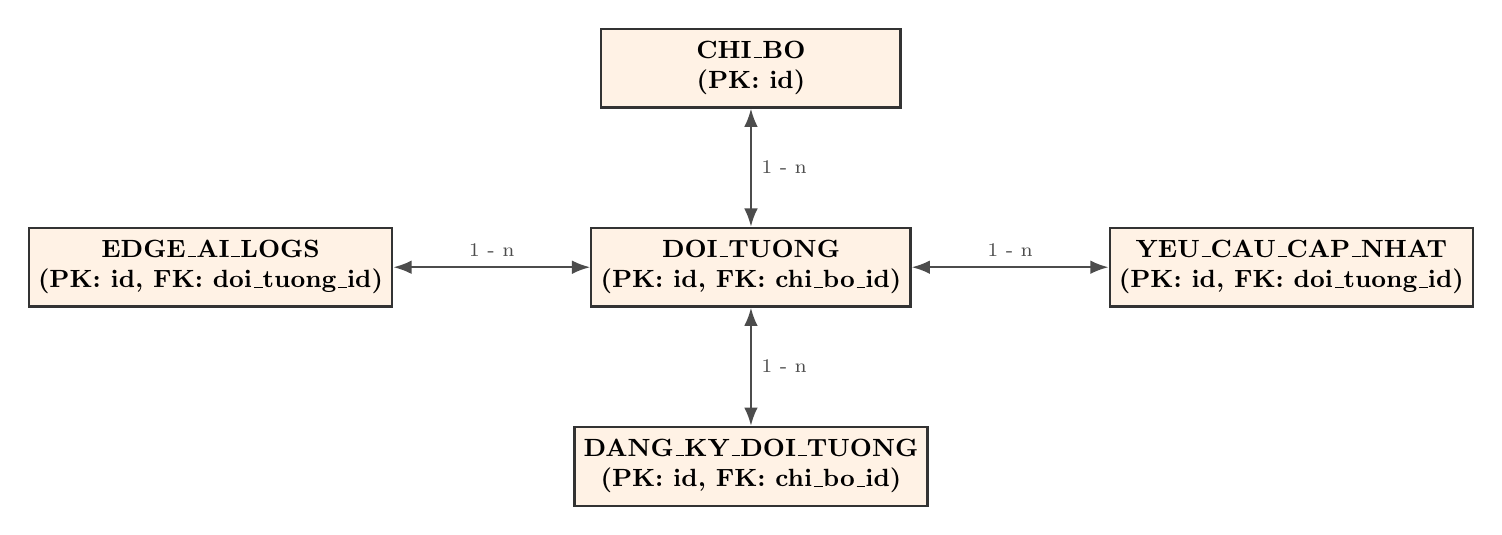
\begin{tikzpicture}[node distance=1.8cm, auto,
          entity/.style={rectangle, draw=black!80, fill=orange!10, thick, minimum width=3.8cm, minimum height=1.0cm, align=center, font=\small\bfseries},
          arrow/.style={Latex-Latex, thick, color=black!70}]

        \node [entity] (doi_tuong) {DOI\_TUONG\\(PK: id, FK: chi\_bo\_id)};
        \node [entity, right=2.5cm of doi_tuong] (yccn) {YEU\_CAU\_CAP\_NHAT\\(PK: id, FK: doi\_tuong\_id)};
        \node [entity, below=1.5cm of doi_tuong] (dkdt) {DANG\_KY\_DOI\_TUONG\\(PK: id, FK: chi\_bo\_id)};
        \node [entity, left=2.5cm of doi_tuong] (ai_logs) {EDGE\_AI\_LOGS\\(PK: id, FK: doi\_tuong\_id)};
        \node [entity, above=1.5cm of doi_tuong] (chi_bo) {CHI\_BO\\(PK: id)};

        \draw [arrow] (doi_tuong) -- node[above, font=\scriptsize]{1 - n} (yccn);
        \draw [arrow] (doi_tuong) -- node[right, font=\scriptsize]{1 - n} (dkdt);
        \draw [arrow] (doi_tuong) -- node[above, font=\scriptsize]{1 - n} (ai_logs);
        \draw [arrow] (chi_bo) -- node[right, font=\scriptsize]{1 - n} (doi_tuong);
      \end{tikzpicture}}
    \vspace{0.4em}
  \end{minipage}
  \caption{Sơ đồ Quan hệ Thực thể ERD Các Bảng Dữ liệu Chính trong Cơ sở Dữ liệu}
  \label{fig:erd_diagram}
\end{figure}

Chứng minh Lược đồ CSDL đạt Dạng chuẩn 3 (3NF):
Một lược đồ quan hệ đạt chuẩn 3NF khi đạt chuẩn 2NF và không chứa phụ thuộc bắc cầu giữa các thuộc tính không khóa vào khóa chính. Để chứng minh thiết kế CSDL \texttt{ql\_dangvien} đạt 3NF, tập các phụ thuộc hàm chính quy ($F$) được xác lập như sau:
\begin{enumerate}[label=\arabic*.]
  \item Bảng \texttt{doi\_tuong}: Khóa chính là $\text{id}$, khóa ứng viên duy nhất là $\text{ma\_gvsv}$.
        \begin{equation}
          \begin{aligned}
            \text{id} & \to \{\text{ma\_gvsv}, \text{ho\_ten}, \text{sdt}, \text{email}, \text{ngay\_sinh}, \text{que\_quan},       \\
                      & \quad\;\;\; \text{chi\_bo\_id}, \text{dang\_vien\_id}, \text{trang\_thai}, \text{avatar}, \text{ghi\_chu}\}
          \end{aligned}
        \end{equation}
        Mọi thuộc tính mô tả cá nhân đều phụ thuộc đầy đủ và trực tiếp vào khóa chính $\text{id}$.
  \item Bảng \texttt{chi\_bo}: $\text{id} \to \{\text{ten\_chi\_bo}, \text{bi\_thu}, \text{email}, \text{dang\_uy}\}$.
  \item Bảng \texttt{dang\_vien}: $\text{id} \to \{\text{ho\_ten}, \text{chi\_bo\_id}, \text{sdt}, \text{chuc\_vu}, \text{ngay\_vao}\}$.
  \item Bảng \texttt{nguoi\_dung}: $\text{id} \to \{\text{user}, \text{pass\_hash}, \text{ho\_ten}, \text{role}\}; \; \text{user} \to \text{id}$.
  \item Bảng \texttt{yeu\_cau\_cap\_nhat}: $\text{id} \to \{\text{doi\_tuong\_id}, \text{truong\_sua}, \text{cu}, \text{moi}, \text{trang\_thai}\}$.
  \item Bảng \texttt{edge\_ai\_logs}: $\text{id} \to \{\text{doi\_tuong\_id}, \text{loai}, \text{verdict}, \text{ty\_le}, \text{time}\}$.
  \item Bảng \texttt{lich\_su}: $\text{id} \to \{\text{doi\_tuong\_id}, \text{actor\_id}, \text{action}, \text{detail}, \text{time}\}$.
  \item Bảng \texttt{dang\_ky\_doi\_tuong}: $\text{id} \to \{\text{ma\_gvsv}, \text{ho\_ten}, \text{chi\_bo\_id}, \text{sdt}, \text{status}\}$.
  \item Bảng \texttt{cai\_dat}: $\text{id} \to \{\text{ten\_truong}, \text{ten\_dang\_bo}, \text{email}, \text{logo}\}$.
\end{enumerate}

Luận giải Phân tách Bảng và Triệt tiêu Dị thường Dữ liệu:
\begin{itemize}[label=--,leftmargin=*]
  \item \textit{Tách danh mục Chi bộ (\texttt{chi\_bo})}: Nếu lưu trực tiếp tên Bí thư, Đảng ủy trực thuộc vào bảng \texttt{doi\_tuong}, khi Bí thư Chi bộ thay đổi sẽ phải cập nhật hàng trăm bản ghi sinh viên (Dị thường cập nhật - Update Anomaly). Việc tách bảng \texttt{chi\_bo} và liên kết qua khóa ngoại \texttt{chi\_bo\_id} triệt tiêu hoàn toàn sự dư thừa này.
  \item \textit{Tách danh sách Đảng viên (\texttt{dang\_vien})}: Một đảng viên có thể hướng dẫn nhiều quần chúng ưu tú. Việc tách riêng thực thể Đảng viên với khóa ngoại \texttt{dang\_vien\_id} giúp đảm bảo tính toàn vẹn khi thông tin của Đảng viên thay đổi.
  \item \textit{Tách các quan hệ $1 - n$ (\texttt{yeu\_cau\_cap\_nhat}, \texttt{edge\_ai\_logs}, \texttt{lich\_su})}: Một quần chúng có thể gửi nhiều lần đề xuất cập nhật thông tin và thực hiện nhiều lượt quét OCR. Việc lưu trữ các tập bản ghi biến động này trong các bảng riêng biệt với khóa ngoại \texttt{doi\_tuong\_id} đảm bảo không vi phạm chuẩn 1NF (thuộc tính đơn trị) và 3NF.
  \item \textit{Nguyên tắc Xóa mềm (Soft Delete) và Nhật ký Kiểm toán (Audit Trail)}: Để bảo vệ toàn vẹn lịch sử hồ sơ chính trị, hệ thống không xóa vật lý các bản ghi mà sử dụng cờ trạng thái \texttt{trang\_thai = 'da\_xoa'} kết hợp ghi vết thao tác vào bảng \texttt{lich\_su}, đảm bảo khả năng khôi phục và phục vụ công tác thanh tra Đảng vụ.
\end{itemize}

Nhằm trực quan hóa đầy đủ toàn bộ kiến trúc dữ liệu và các ràng buộc toàn vẹn giữa các thực thể, sơ đồ quan hệ thực thể mở rộng bao quát 9 bảng dữ liệu trong hệ thống được thể hiện tại Hình \ref{fig:erd_9_tables}.

-- Phân tích Chi tiết Kiến trúc Dữ liệu và Các Mối Quan hệ Thực thể (Hình \ref{fig:erd_9_tables}):
\begin{figure}[htbp]
  \centering
  \begin{minipage}{\linewidth}
    \centering
    \vspace{0.3em}
    \resizebox{\linewidth}{!}{%
      \begin{tikzpicture}[
          font=\fontsize{7.5pt}{9.5pt}\selectfont,
          tablebox/.style={
              rectangle,
              draw=black!85,
              fill=white,
              thick,
              rounded corners=2pt,
              inner sep=4pt,
              align=center
            },
          maintable/.style={
              rectangle,
              draw=red!85!black,
              fill=white,
              very thick,
              rounded corners=2pt,
              inner sep=4pt,
              align=center
            },
          biarrow/.style={
              {Latex[scale=0.85]}-{Latex[scale=0.85]},
              thick,
              color=black!80
            }
        ]

        % ----------------------------------------------------
        % HÀNG 1: TOP (y = 5.8)
        % ----------------------------------------------------
        \node [tablebox] (nguoi_dung) at (-7.2, 5.8) {
          \begin{tabular}{@{}p{2.8cm} r@{}}
            \multicolumn{2}{c}{\textbf{\normalsize NGUOI\_DUNG}} \\
            \hline
            \textbf{id}    & \textit{[PK]}                       \\
            username       & \textit{[UK]}                       \\
            password\_hash &                                     \\
            ho\_ten        &                                     \\
            vai\_tro       &                                     \\
          \end{tabular}
        };

        \node [tablebox] (chi_bo) at (0.0, 5.8) {
          \begin{tabular}{@{}p{2.8cm} r@{}}
            \multicolumn{2}{c}{\textbf{\normalsize CHI\_BO}} \\
            \hline
            \textbf{id}    & \textit{[PK]}                   \\
            ten\_chi\_bo   &                                 \\
            bi\_thu        &                                 \\
            email\_chi\_bo &                                 \\
            dang\_uy       &                                 \\
          \end{tabular}
        };

        \node [tablebox] (dang_vien) at (7.2, 5.8) {
          \begin{tabular}{@{}p{2.8cm} r@{}}
            \multicolumn{2}{c}{\textbf{\normalsize DANG\_VIEN}} \\
            \hline
            \textbf{id}    & \textit{[PK]}                      \\
            chi\_bo\_id    & \textit{[FK]}                      \\
            ho\_ten        &                                    \\
            chuc\_vu       &                                    \\
            sdt, ngay\_vao &                                    \\
          \end{tabular}
        };

        % ----------------------------------------------------
        % HÀNG 2: MIDDLE (y = 0.0)
        % ----------------------------------------------------
        \node [tablebox] (dkdt) at (-7.2, 0.0) {
          \begin{tabular}{@{}p{3.2cm} r@{}}
            \multicolumn{2}{c}{\textbf{\normalsize DANG\_KY\_DOI\_TUONG}} \\
            \hline
            \textbf{id}         & \textit{[PK]}                           \\
            chi\_bo\_id         & \textit{[FK]}                           \\
            ma\_gvsv, ho\_ten   &                                         \\
            sdt, email, lop     &                                         \\
            trang\_thai, ly\_do &                                         \\
          \end{tabular}
        };

        \node [maintable] (doi_tuong) at (0.0, 0.0) {
          \begin{tabular}{@{}p{3.8cm} r@{}}
            \multicolumn{2}{c}{\textbf{\normalsize\color{red!85!black}DOI\_TUONG (Hạt nhân)}} \\
            \hline
            \textbf{id}                    & \textit{[PK]}                                    \\
            \textbf{ma\_gvsv}              & \textit{[UK]}                                    \\
            chi\_bo\_id, dang\_vien\_id    & \textit{[FK]}                                    \\
            ho\_ten, sdt, email            &                                                  \\
            ngay\_sinh, que\_quan, lop     &                                                  \\
            gioi\_tinh, dan\_toc, chuc\_vu &                                                  \\
            so\_bc\_cam\_tinh, ngay\_hop   &                                                  \\
            dang\_vien\_giup\_do           &                                                  \\
            so\_qd\_cc, ngay\_cap\_cc      &                                                  \\
            ket\_nap\_dang, ngay\_kn       &                                                  \\
            trang\_thai, avatar, ghi\_chu  &                                                  \\
          \end{tabular}
        };

        \node [tablebox] (yccn) at (7.2, 0.0) {
          \begin{tabular}{@{}p{3.2cm} r@{}}
            \multicolumn{2}{c}{\textbf{\normalsize YEU\_CAU\_CAP\_NHAT}} \\
            \hline
            \textbf{id}         & \textit{[PK]}                          \\
            doi\_tuong\_id      & \textit{[FK]}                          \\
            sdt, email, lop     &                                        \\
            que\_quan, chuc\_vu &                                        \\
            trang\_thai, ly\_do &                                        \\
          \end{tabular}
        };

        % ----------------------------------------------------
        % HÀNG 3: BOTTOM (y = -5.8)
        % ----------------------------------------------------
        \node [tablebox] (lich_su) at (-7.2, -5.8) {
          \begin{tabular}{@{}p{2.8cm} r@{}}
            \multicolumn{2}{c}{\textbf{\normalsize LICH\_SU}} \\
            \hline
            \textbf{id}       & \textit{[PK]}                 \\
            doi\_tuong\_id    & \textit{[FK]}                 \\
            hanh\_dong        &                               \\
            mo\_ta            &                               \\
            nguoi\_thuc\_hien &                               \\
            thoi\_gian        &                               \\
          \end{tabular}
        };

        \node [tablebox] (ai_logs) at (0.0, -5.8) {
          \begin{tabular}{@{}p{2.8cm} r@{}}
            \multicolumn{2}{c}{\textbf{\normalsize EDGE\_AI\_LOGS}} \\
            \hline
            \textbf{id}          & \textit{[PK]}                    \\
            doi\_tuong\_id       & \textit{[FK]}                    \\
            loai\_phieu, verdict &                                  \\
            ty\_le\_hoan\_thien  &                                  \\
            raw\_summary, files  &                                  \\
          \end{tabular}
        };

        \node [tablebox] (cai_dat) at (7.2, -5.8) {
          \begin{tabular}{@{}p{2.8cm} r@{}}
            \multicolumn{2}{c}{\textbf{\normalsize CAI\_DAT}} \\
            \hline
            \textbf{id}     & \textit{[PK]}                   \\
            ten\_truong     &                                 \\
            ten\_dang\_bo   &                                 \\
            email\_lien\_he &                                 \\
            dia\_chi, logo  &                                 \\
          \end{tabular}
        };

        % ----------------------------------------------------
        % CÁC ĐƯỜNG LIÊN KẾT QUAN HỆ (KHÔNG GIAO CẮT BẢNG)
        % ----------------------------------------------------
        % 1. Chi bộ -> Đảng viên
        \draw [biarrow] (chi_bo.east) -- node[above, font=\fontsize{6.5pt}{8pt}\selectfont]{Quản lý ĐV} node[pos=0.08, below, font=\scriptsize\bfseries]{1} node[pos=0.92, below, font=\scriptsize\bfseries]{n} (dang_vien.west);

        % 2. Chi bộ -> Đối tượng
        \draw [biarrow] (chi_bo.south) -- node[right, font=\fontsize{6.5pt}{8pt}\selectfont]{Quản lý hồ sơ} node[pos=0.08, left, font=\scriptsize\bfseries]{1} node[pos=0.92, left, font=\scriptsize\bfseries]{n} (doi_tuong.north);

        % 3. Chi bộ -> Đăng ký đối tượng
        \draw [biarrow] (chi_bo.south west) -- node[above, font=\fontsize{6.5pt}{8pt}\selectfont, sloped]{Tiếp nhận đơn} node[pos=0.15, above, font=\scriptsize\bfseries]{1} node[pos=0.85, above, font=\scriptsize\bfseries]{n} (dkdt.north east);

        % 4. Đảng viên -> Đối tượng
        \draw [biarrow] (dang_vien.south west) -- node[above, font=\fontsize{6.5pt}{8pt}\selectfont, sloped]{Phân công giúp đỡ} node[pos=0.15, above, font=\scriptsize\bfseries]{1} node[pos=0.85, above, font=\scriptsize\bfseries]{n} (doi_tuong.north east);

        % 5. Người dùng -> Đăng ký đối tượng (Thẳng đứng, không cắt qua bảng khác)
        \draw [biarrow] (nguoi_dung.south) -- node[left, font=\fontsize{6.5pt}{8pt}\selectfont, align=center]{Nộp hồ sơ\\trực tuyến} node[pos=0.08, right, font=\scriptsize\bfseries]{1} node[pos=0.92, right, font=\scriptsize\bfseries]{n} (dkdt.north);

        % 6. Người dùng -> Lịch sử (Bo cung bên mép ngoài bên trái)
        \draw [biarrow] (nguoi_dung.west) to[out=180, in=180] node[left, font=\fontsize{6.5pt}{8pt}\selectfont]{Người thực hiện} node[pos=0.05, below, font=\scriptsize\bfseries]{1} node[pos=0.95, above, font=\scriptsize\bfseries]{n} (lich_su.west);

        % 7. Đối tượng -> Yêu cầu cập nhật
        \draw [biarrow] (doi_tuong.east) -- node[above, font=\fontsize{6.5pt}{8pt}\selectfont]{Đề xuất sửa} node[pos=0.08, below, font=\scriptsize\bfseries]{1} node[pos=0.92, below, font=\scriptsize\bfseries]{n} (yccn.west);

        % 8. Đối tượng -> Nhật ký AI
        \draw [biarrow] (doi_tuong.south) -- node[right, font=\fontsize{6.5pt}{8pt}\selectfont]{Lưu nhật ký AI} node[pos=0.08, left, font=\scriptsize\bfseries]{1} node[pos=0.92, left, font=\scriptsize\bfseries]{n} (ai_logs.north);

        % 9. Đối tượng -> Lịch sử
        \draw [biarrow] (doi_tuong.south west) -- node[above, font=\fontsize{6.5pt}{8pt}\selectfont, sloped]{Ghi vết kiểm toán} node[pos=0.15, above, font=\scriptsize\bfseries]{1} node[pos=0.85, above, font=\scriptsize\bfseries]{n} (lich_su.north east);

      \end{tikzpicture}}
    \vspace{0.3em}
  \end{minipage}
  \caption{Sơ đồ Quan hệ Thực thể ERD Mở rộng Toàn diện 9 Bảng Dữ liệu trong CSDL ql\_dangvien}
  \label{fig:erd_9_tables}
\end{figure}
Sơ đồ ERD tại Hình \ref{fig:erd_9_tables} mô hình hóa toàn diện cấu trúc cơ sở dữ liệu \texttt{ql\_dangvien} gồm 9 bảng được phân chia thành 5 nhóm chức năng nghiệp vụ chặt chẽ:
\begin{enumerate}[label=\arabic*.]
  \item Thực thể Hạt nhân Trung tâm (\texttt{doi\_tuong}): Đóng vai trò cốt lõi lưu trữ toàn bộ tiến trình rèn luyện và 35 trường thông tin cá nhân, hành chính của quần chúng ưu tú. Bảng sở hữu khóa chính $\text{id}$ cùng khóa duy nhất (\texttt{UNIQUE}) $\text{ma\_gvsv}$, đảm bảo tính toàn vẹn và ngăn chặn tuyệt đối tình trạng trùng lặp hồ sơ trong hệ thống.
  \item Nhóm Thực thể Danh mục và Phân quyền (\texttt{chi\_bo}, \texttt{dang\_vien}, \texttt{nguoi\_dung}):
        \begin{itemize}[label=--,leftmargin=*]
          \item \texttt{chi\_bo}: Lưu trữ danh mục các Chi bộ Đảng trực thuộc Đảng ủy Trường, liên kết với \texttt{doi\_tuong} qua khóa ngoại \texttt{chi\_bo\_id} với quan hệ $1 - n$ (Một Chi bộ quản lý theo dõi nhiều Quần chúng ưu tú).
          \item \texttt{dang\_vien}: Lưu danh sách Đảng viên chính thức, liên kết với \texttt{doi\_tuong} qua khóa ngoại \texttt{dang\_vien\_id} với quan hệ $1 - n$ (Một Đảng viên chính thức có thể được phân công giúp đỡ nhiều Quần chúng).
          \item \texttt{nguoi\_dung}: Đảm nhiệm xác thực tài khoản và phân quyền RBAC (Sinh viên, Bí thư, Admin), liên kết với quy trình nộp đơn và nhật ký thao tác.
        \end{itemize}
  \item Nhóm Thực thể Vùng đệm Xét duyệt (\texttt{dang\_ky\_doi\_tuong}, \texttt{yeu\_cau\_cap\_nhat}):
        \begin{itemize}[label=--,leftmargin=*]
          \item \texttt{dang\_ky\_doi\_tuong}: Đóng vai trò là hàng chờ (Staging Buffer) tiếp nhận đơn đăng ký trực tuyến từ tài khoản \texttt{nguoi\_dung} và chuyển tiếp tới Chi bộ đề xuất. Dữ liệu chỉ được chuyển vào bảng chính thức \texttt{doi\_tuong} sau khi Bí thư Chi bộ thẩm định và phê duyệt.
          \item \texttt{yeu\_cau\_cap\_nhat}: Tiếp nhận các đề xuất thay đổi thông tin cá nhân (SĐT, Email, Lớp, Quê quán) do Quần chúng gửi lên, liên kết trực tiếp với bảng \texttt{doi\_tuong} qua khóa ngoại \texttt{doi\_tuong\_id}. Bảng này cung cấp dữ liệu phục vụ giao diện đối chiếu 2 tab Cũ -- Mới của Bí thư trước khi cập nhật dữ liệu.
        \end{itemize}
  \item Nhóm Thực thể Kiểm toán và Nhật ký AI (\texttt{lich\_su}, \texttt{edge\_ai\_logs}):
        \begin{itemize}[label=--,leftmargin=*]
          \item \texttt{lich\_su}: Lưu vết bất biến (Audit Trail) mọi thao tác Thêm, Sửa, Xóa, Duyệt trong hệ thống, ghi nhận mã định danh người thực hiện (\texttt{nguoi\_dung}) và hồ sơ chịu tác động (\texttt{doi\_tuong}).
          \item \texttt{edge\_ai\_logs}: Lưu trữ lịch sử thẩm định của phân hệ Edge AI OCR, bao gồm loại phiếu minh chứng, phán quyết kỹ thuật \texttt{agentVerdict}, tỷ lệ hoàn thiện \% và đường dẫn tệp tài liệu lưu tại thư mục \texttt{uploads/ho\_so\_minh\_chung/}.
        \end{itemize}
  \item Thực thể Cấu hình Hệ thống Toàn cục (\texttt{cai\_dat}): Lưu trữ các tham số hệ thống chung (Tên Trường, Tên Đảng bộ, Email liên hệ, Logo) áp dụng thống nhất cho toàn bộ hệ thống giao diện và phân hệ kết xuất 8 mẫu phiếu PDF/Excel.
\end{enumerate}

Nguyên tắc Đảm bảo Toàn vẹn Dữ liệu và Triệt tiêu Dị thường:
Toàn bộ các mối quan hệ $1 - n$ được thiết lập qua các ràng buộc Khóa ngoại (Foreign Keys) với cơ chế \texttt{ON DELETE RESTRICT} và \texttt{ON UPDATE CASCADE}. Thiết kế này đảm bảo không làm phát sinh dữ liệu mồ côi (Orphan Records) khi có thay đổi danh mục, đồng thời kết hợp cơ chế xóa mềm (\texttt{trang\_thai = 'da\_xoa'}) giúp duy trì trọn vẹn lịch sử hồ sơ Đảng vụ phục vụ công tác thanh tra và kiểm toán chính trị.

\subsection*{5.2 Từ điển dữ liệu chi tiết 9 bảng CSDL MySQL (Data Dictionary)}
\addcontentsline{toc}{subsection}{5.2 Từ điển dữ liệu chi tiết 9 bảng CSDL MySQL (Data Dictionary)}
Toàn bộ cơ sở dữ liệu \texttt{ql\_dangvien} được cấu thành từ đúng 9 bảng dữ liệu chuẩn hóa. Trong đó, bảng chính \texttt{doi\_tuong} chứa 35 cột thông tin hồ sơ được mô tả tại Bảng \ref{tab:doi_tuong_schema}:

{\setstretch{1.25}\fontsize{9pt}{11.5pt}\selectfont
  \begin{xltabular}{\linewidth}{|>{\raggedright\arraybackslash}p{4.8cm}|>{\raggedright\arraybackslash}p{2.8cm}|>{\raggedright\arraybackslash}X|}
    \caption{Đặc tả bảng dữ liệu chính doi\_tuong (35 cột dữ liệu hồ sơ quần chúng)} \label{tab:doi_tuong_schema} \\
    \hline
    \textbf{Tên Cột} & \textbf{Kiểu Dữ liệu} & \textbf{Mô tả Ý nghĩa Nghiệp vụ} \\ \hline
    \endfirsthead
    \multicolumn{3}{c}{\textit{(Tiếp theo Bảng \ref{tab:doi_tuong_schema})}} \\ \hline
    \textbf{Tên Cột} & \textbf{Kiểu Dữ liệu} & \textbf{Mô tả Ý nghĩa Nghiệp vụ} \\ \hline
    \endhead
    \hline
    \endfoot
    \texttt{id}                                          & INT PK Auto   & Mã định danh tự tăng duy nhất của hồ sơ                        \\ \hline
    \texttt{ma\_gvsv}                                    & VARCHAR(50)   & Mã số Sinh viên / Giảng viên (Khóa duy nhất)                   \\ \hline
    \texttt{ho\_ten}                                     & VARCHAR(255)  & Họ và tên đầy đủ quần chúng                                    \\ \hline
    \texttt{sdt}, \texttt{email}                         & VARCHAR       & Số điện thoại và Địa chỉ Email liên hệ                         \\ \hline
    \texttt{gioi\_tinh}, \texttt{ngay\_sinh}             & VARCHAR, DATE & Giới tính và Ngày tháng năm sinh                               \\ \hline
    \texttt{dan\_toc}, \texttt{que\_quan}                & VARCHAR, TEXT & Dân tộc và Địa chỉ Quê quán                                    \\ \hline
    \texttt{chuc\_vu}, \texttt{lop}                      & VARCHAR       & Chức vụ Đoàn/Lớp và Lớp sinh hoạt hành chính                   \\ \hline
    \texttt{chi\_bo\_cong\_nhan}                         & VARCHAR(255)  & Tên Chi bộ Đảng theo dõi công nhận (Liên kết \texttt{chi\_bo}) \\ \hline
    \texttt{so\_bc\_cam\_tinh}                           & VARCHAR(50)   & Số biên bản họp công nhận cảm tình Đảng                        \\ \hline
    \texttt{ngay\_hop\_cam\_tinh}                        & DATE          & Ngày Chi bộ họp công nhận cảm tình Đảng                        \\ \hline
    \texttt{dang\_vien\_giup\_do}                        & VARCHAR(255)  & Họ tên Đảng viên chính thức được phân công giúp đỡ             \\ \hline
    \texttt{ngay\_phan\_cong\_giup\_do}                  & DATE          & Ngày Chi bộ ra quyết định phân công giúp đỡ                    \\ \hline
    \texttt{so\_qd\_mo\_lop}, \texttt{ngay\_qd\_mo\_lop} & VARCHAR, DATE & Số và Ngày quyết định mở lớp nhận thức về Đảng                 \\ \hline
    \texttt{tg\_lop\_boi\_duong}                         & VARCHAR(100)  & Thời gian tham gia lớp bồi dưỡng nhận thức về Đảng             \\ \hline
    \texttt{ngay\_cap\_cc}, \texttt{so\_qd\_cc}          & DATE, VARCHAR & Ngày và Số quyết định cấp Chứng chỉ nhận thức về Đảng          \\ \hline
    \texttt{don\_vi\_cap\_cc}                            & VARCHAR(255)  & Đơn vị cấp Chứng chỉ (Trung tâm chính trị / Trường)            \\ \hline
    \texttt{ten\_chibo\_khi\_cap\_cc}                    & VARCHAR(255)  & Tên Chi bộ sinh hoạt tại thời điểm cấp Chứng chỉ               \\ \hline
    \texttt{ten\_danguy\_khi\_cap\_cc}                   & VARCHAR(255)  & Tên Đảng ủy quản lý tại thời điểm cấp Chứng chỉ                \\ \hline
    \texttt{ket\_nap\_dang}, \texttt{so\_qd\_ket\_nap}   & VARCHAR       & Trạng thái kết nạp và Số quyết định kết nạp Đảng               \\ \hline
    \texttt{ngay\_quyet\_dinh}, \texttt{ngay\_ket\_nap}  & DATE, DATE    & Ngày ký quyết định và Ngày tổ chức lễ kết nạp                  \\ \hline
    \texttt{dang\_vien\_huong\_dan}                      & VARCHAR(255)  & Đảng viên chính thức hướng dẫn 12 tháng dự bị                  \\ \hline
    \texttt{ngay\_chuyen\_sinh\_hoat}                    & DATE          & Ngày làm thủ tục chuyển sinh hoạt Đảng chính thức              \\ \hline
    \texttt{noi\_chuyen\_toi}                            & VARCHAR(255)  & Chi bộ / Đảng bộ nơi chuyển sinh hoạt tới                      \\ \hline
    \texttt{trang\_thai}                                 & VARCHAR(50)   & Trạng thái: 'Đang theo dõi', 'Đã kết nạp', 'Đã chuyển'         \\ \hline
    \texttt{avatar}                                      & VARCHAR(255)  & Đường dẫn ảnh chân dung lưu tại uploads/avatars/               \\ \hline
    \texttt{ghi\_chu}                                    & TEXT          & Ghi chú bổ sung của Bí thư Chi bộ                              \\ \hline
  \end{xltabular}}

Phân tích cấu trúc bảng dữ liệu chính \texttt{doi\_tuong}: Bảng \texttt{doi\_tuong} (Bảng \ref{tab:doi_tuong_schema}) đóng vai trò hạt nhân trong lược đồ CSDL, lưu trữ 35 thuộc tính nghiệp vụ trải dài qua toàn bộ vòng đời xét duyệt kết nạp. Các trường khóa và chỉ mục (Index) được thiết lập tối ưu: \texttt{ma\_gvsv} là khóa duy nhất (\texttt{UNIQUE INDEX}), các trường \texttt{chi\_bo\_cong\_nhan}, \texttt{trang\_thai} và \texttt{email} được đánh chỉ mục (\texttt{BTREE INDEX}) để tăng tốc các truy vấn tìm kiếm và lọc danh sách. Cơ chế xóa mềm (Soft Delete) được áp dụng qua trường \texttt{trang\_thai} nhằm bảo tồn toàn vẹn dữ liệu lịch sử Đảng viên và ngăn chặn thất thoát dữ liệu do thao tác xóa nhầm.

Đặc tả 8 bảng dữ liệu phụ thuộc còn lại trong hệ thống được liệt kê chi tiết tại Bảng \ref{tab:sub_tables_schema}:

Phân tích mối quan hệ giữa 8 bảng dữ liệu phụ thuộc: Cấu trúc 8 bảng phụ thuộc tại Bảng \ref{tab:sub_tables_schema} hoàn thiện tính toàn vẹn dữ liệu cho lược đồ CSDL chuẩn 3NF. Bảng \texttt{dang\_ky\_doi\_tuong} và \texttt{yeu\_cau\_cap\_nhat} đóng vai trò là vùng đệm (Staging Buffer) chứa dữ liệu đầu vào trước khi được Bí thư xác nhận chuyển vào bảng chính \texttt{doi\_tuong}. Bảng \texttt{edge\_ai\_logs} và \texttt{lich\_su} thiết lập cơ chế kiểm toán vết (Audit Trail) ghi lại mọi thao tác của người dùng và phán quyết của AI Agents. Quy trình chuyển đổi trạng thái hồ sơ tuân thủ máy trạng thái hữu hạn (Finite State Machine): $\text{Chờ duyệt} \to \text{Cảm tình Đảng} \to \text{Học lớp nhận thức} \to \text{Đảng viên dự bị} \to \text{Đảng viên chính thức}$. Các ràng buộc Khóa ngoại (Foreign Keys) với cơ chế \texttt{ON DELETE RESTRICT} ngăn chặn hiện tượng dữ liệu mồ côi khi xóa tài khoản hay chi bộ.
  {\setstretch{1.25}\fontsize{9pt}{11.5pt}\selectfont
    \begin{xltabular}{\linewidth}{|c|>{\raggedright\arraybackslash}p{4.2cm}|>{\raggedright\arraybackslash}p{2.3cm}|>{\raggedright\arraybackslash}X|}
      \caption{Đặc tả 8 Bảng Dữ liệu Phụ thuộc trong Cơ sở Dữ liệu ql\_dangvien} \label{tab:sub_tables_schema} \\
      \hline
      \textbf{STT} & \textbf{Tên Bảng CSDL} & \textbf{Khóa Chính} & \textbf{Chức năng \& Ý nghĩa Lưu trữ Dữ liệu} \\ \hline
      \endfirsthead
      \multicolumn{4}{c}{\textit{(Tiếp theo Bảng \ref{tab:sub_tables_schema})}} \\ \hline
      \textbf{STT} & \textbf{Tên Bảng CSDL} & \textbf{Khóa Chính} & \textbf{Chức năng \& Ý nghĩa Lưu trữ Dữ liệu} \\ \hline
      \endhead
      \hline
      \endfoot
      1 & \texttt{nguoi\_dung}          & \texttt{id} & Tài khoản người dùng (username, password băm BCRYPT, role) \\ \hline
      2 & \texttt{dang\_ky\_doi\_tuong} & \texttt{id} & Đơn đăng ký quần chúng mới chờ Bí thư duyệt                \\ \hline
      3 & \texttt{yeu\_cau\_cap\_nhat}  & \texttt{id} & Đề xuất chỉnh sửa thông tin cá nhân chờ Bí thư duyệt       \\ \hline
      4 & \texttt{chi\_bo}              & \texttt{id} & Danh mục các Chi bộ Đảng trực thuộc Đảng ủy Trường         \\ \hline
      5 & \texttt{dang\_vien}           & \texttt{id} & Danh sách Đảng viên chính thức phân công giúp đỡ           \\ \hline
      6 & \texttt{edge\_ai\_logs}       & \texttt{id} & Nhật ký kiểm tra OCR, agentVerdict \& actionAdvice của AI  \\ \hline
      7 & \texttt{lich\_su}             & \texttt{id} & Lịch sử thao tác hệ thống (Audit Trail Logging)            \\ \hline
      8 & \texttt{cai\_dat}             & \texttt{id} & Cấu hình hằng số hệ thống (Tên Trường, Email, Logo)        \\ \hline
    \end{xltabular}}
\subsection*{5.3 Nhận dạng CCCD tự điền form và cắt ảnh thẻ Canvas 3x4}
\addcontentsline{toc}{subsection}{5.3 Nhận dạng CCCD tự điền form và cắt ảnh thẻ Canvas 3x4}
Dựa trên cấu trúc dữ liệu đã được chuẩn hóa 3NF, các kịch bản tương tác động giữa người dùng, trình duyệt và các dịch vụ backend được mô tả tuần tự qua 4 quy trình cốt lõi. Sơ đồ tuần tự tại Hình \ref{fig:seq_autofill} mô tả chi tiết tương tác giữa Sinh viên, Trình duyệt Web, Engine OCR Tesseract.js và Canvas Crop 3x4.

\begin{figure}[htbp]
  \centering
  \begin{minipage}{\linewidth}
    \centering
    \vspace{0.4em}
    \resizebox{\linewidth}{!}{%
      \begin{tikzpicture}[node distance=0.45cm, auto, font=\small,
          stepbox/.style={rectangle, draw=blue!70!black, fill=blue!5, thick, minimum width=13.5cm, minimum height=0.75cm, align=left, rounded corners=3pt},
          arrow/.style={-Latex, thick, color=blue!80!black}]
        \node [stepbox] (s1) {Bước 1: Sinh viên $\rightarrow$ Chọn tệp ảnh CCCD/Thẻ SV tải lên Giao diện Web};
        \node [stepbox, below=0.3cm of s1] (s2) {Bước 2: Giao diện Web $\rightarrow$ Nạp mảng byte dữ liệu sang Worker \texttt{Tesseract.js} (WASM)};
        \node [stepbox, below=0.3cm of s2] (s3) {Bước 3: Tesseract.js Engine $\rightarrow$ Giải mã ký tự quang học \& Trả về chuỗi văn bản raw};
        \node [stepbox, below=0.3cm of s3] (s4) {Bước 4: Giao diện Web $\rightarrow$ Chạy Regex khớp thông tin \& Auto-fill vào các trường Form};
        \node [stepbox, below=0.3cm of s4] (s5) {Bước 5: Sinh viên $\rightarrow$ Tải ảnh đại diện chân dung lên mô đun Cắt ảnh Canvas};
        \node [stepbox, below=0.3cm of s5] (s6) {Bước 6: HTML5 Canvas $\rightarrow$ Nhận diện khuôn mặt, cắt chuẩn 3x4 ($300 \times 400$px) \& Xuất Base64};

        \draw [arrow] (s1) -- (s2);
        \draw [arrow] (s2) -- (s3);
        \draw [arrow] (s3) -- (s4);
        \draw [arrow] (s4) -- (s5);
        \draw [arrow] (s5) -- (s6);
      \end{tikzpicture}}
    \vspace{0.4em}
  \end{minipage}
  \caption{Sơ đồ Tuần tự Quy trình OCR Trích xuất CCCD và Smart Canvas Crop Ảnh 3x4}
  \label{fig:seq_autofill}
\end{figure}

Phân tích logic quy trình OCR và Crop ảnh: Quy trình tại Hình \ref{fig:seq_autofill} tự động hóa các thao tác nhập liệu ban đầu của Sinh viên. Khi người dùng nạp ảnh CCCD mặt trước/mặt sau, Giao diện Web nạp dữ liệu ảnh dạng mảng byte sang Worker \texttt{Tesseract.js} chạy trong luồng ngầm (Web Worker WASM). Engine \texttt{Tesseract.js} giải mã văn bản hình ảnh và trả về chuỗi ký tự thô. Giao diện Web lập tức chạy thuật toán biểu thức chính quy (Regex) để trích xuất các trường thông tin: Họ tên, Số CCCD, Ngày sinh, Quê quán và tự động nạp (auto-fill) vào form đăng ký. Tiếp đó, khi sinh viên tải ảnh chân dung, thư viện Canvas HTML5 tự động xác định vùng khuôn mặt, thực hiện crop theo tỉ lệ 3:4 chuẩn kích thước $300 \times 400$ pixel và mã hóa dạng Base64 để gửi về lưu trữ tại server.

\subsection*{5.4 Thẩm định hồ sơ minh chứng qua hệ thống Multi-Agent AI}
\addcontentsline{toc}{subsection}{5.4 Thẩm định hồ sơ minh chứng qua hệ thống Multi-Agent AI}
Sau khi thông tin định danh ban đầu được lưu trữ, quy trình nghiệp vụ tiếp theo là thẩm định tính đầy đủ của các tệp hồ sơ minh chứng thông qua sự phối hợp giữa Client, Multi-Agent AI Suite và CSDL. Sơ đồ tuần tự tại Hình \ref{fig:seq_multi_agent} mô tả chi tiết luồng thực thi này.

\begin{figure}[htbp]
  \centering
  \begin{minipage}{\linewidth}
    \centering
    \vspace{0.4em}
    \resizebox{\linewidth}{!}{%
      \begin{tikzpicture}[node distance=0.45cm, auto, font=\small,
          stepbox/.style={rectangle, draw=cyan!70!black, fill=cyan!5, thick, minimum width=13.5cm, minimum height=0.75cm, align=left, rounded corners=3pt},
          arrow/.style={-Latex, thick, color=cyan!80!black}]
        \node [stepbox] (s1) {Bước 1: Người dùng $\rightarrow$ Chọn tệp hồ sơ PDF/Scan tải lên giao diện thẩm định};
        \node [stepbox, below=0.3cm of s1] (s2) {Bước 2: Browser Engine $\rightarrow$ Đọc mảng byte và trích xuất nội dung văn bản qua \texttt{PDF.js}};
        \node [stepbox, below=0.3cm of s2] (s3) {Bước 3: Synopsis \& Gap Diagnostic Agents $\rightarrow$ Bóc tách nhãn trường \& Chẩn đoán trường khuyết};
        \node [stepbox, below=0.3cm of s4] (s4) {Bước 4: Executive Agent $\rightarrow$ Tổng hợp \% hoàn thiện, tạo \texttt{agentVerdict} \& \texttt{actionAdvice}};
        \node [stepbox, below=0.3cm of s4] (s5) {Bước 5: Browser Engine $\rightarrow$ Gửi request AJAX \texttt{api\_save\_ai\_check} về Backend PHP};
        \node [stepbox, below=0.3cm of s5] (s6) {Bước 6: Backend PHP PDO $\rightarrow$ Ghi nhận xét đánh giá và nhật ký kiểm tra vào bảng \texttt{edge\_ai\_logs}};

        \draw [arrow] (s1) -- (s2);
        \draw [arrow] (s2) -- (s3);
        \draw [arrow] (s3) -- (s4);
        \draw [arrow] (s4) -- (s5);
        \draw [arrow] (s5) -- (s6);
      \end{tikzpicture}}
    \vspace{0.4em}
  \end{minipage}
  \caption{Sơ đồ Tuần tự Quy trình Multi-Agent AI Thẩm định Hồ sơ và Ghi Log CSDL}
  \label{fig:seq_multi_agent}
\end{figure}

Phân tích logic quy trình thẩm định và lưu log CSDL: Quy trình tại Hình \ref{fig:seq_multi_agent} mô tả sự tương tác giữa Client Browser, Multi-Agent AI Suite và CSDL MySQL qua Backend PHP. Khi người dùng nạp tệp hồ sơ PDF, thư viện \texttt{PDF.js} tại trình duyệt giải mã nội dung văn bản. Bộ đôi Synopsis Agent và Gap Diagnostic Agent tiếp nhận chuỗi dữ liệu để bóc tách thông tin và phát hiện các mục còn khuyết. Executive Agent tổng hợp kết quả đánh giá, sinh ra thông điệp \texttt{agentVerdict} và tỷ lệ hoàn thành. Ngay sau đó, trình duyệt tự động khởi tạo truy vấn AJAX gửi payload JSON chứa thông số thẩm định đến script \texttt{api\_save\_ai\_check.php}. Backend PHP sử dụng PDO Prepared Statements để ghi nhận xét và nhật ký đánh giá vào bảng \texttt{edge\_ai\_logs} trong CSDL MySQL một cách an toàn.

\subsection*{5.5 Đề xuất cập nhật thông tin và phê duyệt đối chiếu 2 Tab}
\addcontentsline{toc}{subsection}{5.5 Đề xuất cập nhật thông tin và phê duyệt đối chiếu 2 Tab}
Bên cạnh khâu thẩm định hồ sơ mới, hệ thống đảm bảo tính toàn vẹn và cập nhật dữ liệu liên tục trong suốt quá trình rèn luyện thông qua quy trình đề xuất cập nhật và phê duyệt đối chiếu 2 tab. Sơ đồ tuần tự tại Hình \ref{fig:seq_approval} thể hiện luồng gửi yêu cầu cập nhật của Sinh viên và thao tác phê duyệt đối chiếu 2 tab của Bí thư Chi bộ.

\begin{figure}[htbp]
  \centering
  \begin{minipage}{\linewidth}
    \centering
    \vspace{0.4em}
    \resizebox{\linewidth}{!}{%
      \begin{tikzpicture}[node distance=0.45cm, auto, font=\small,
          stepbox/.style={rectangle, draw=green!60!black, fill=green!5, thick, minimum width=13.5cm, minimum height=0.75cm, align=left, rounded corners=3pt},
          arrow/.style={-Latex, thick, color=green!70!black}]
        \node [stepbox] (s1) {Bước 1: Sinh viên $\rightarrow$ Nhập thông tin thay đổi (SĐT, Email, Lớp) trên Form đề xuất};
        \node [stepbox, below=0.3cm of s1] (s2) {Bước 2: Giao diện Client $\rightarrow$ Đẩy dữ liệu vào bảng tạm \texttt{yeu\_cau\_cap\_nhat} với trạng thái Chờ duyệt};
        \node [stepbox, below=0.3cm of s2] (s3) {Bước 3: Bí thư Chi bộ $\rightarrow$ Truy cập phân hệ duyệt, mở giao diện đối chiếu 2 Tab (Cũ vs Mới)};
        \node [stepbox, below=0.3cm of s3] (s4) {Bước 4: Hệ thống Web $\rightarrow$ Tô màu vàng nổi bật các ô dữ liệu có sự thay đổi giữa 2 phiên bản};
        \node [stepbox, below=0.3cm of s4] (s5) {Bước 5: Bí thư Chi bộ $\rightarrow$ Xóa/Duyệt đề xuất (Bấm nút Phê duyệt chính thức)};
        \node [stepbox, below=0.3cm of s5] (s6) {Bước 6: Backend PHP $\rightarrow$ Cập nhật dữ liệu mới vào CSDL \texttt{doi\_tuong} \& Lưu vết Lịch sử};

        \draw [arrow] (s1) -- (s2);
        \draw [arrow] (s2) -- (s3);
        \draw [arrow] (s3) -- (s4);
        \draw [arrow] (s4) -- (s5);
        \draw [arrow] (s5) -- (s6);
      \end{tikzpicture}}
    \vspace{0.4em}
  \end{minipage}
  \caption{Sơ đồ Tuần tự Quy trình Đề xuất Cập nhật Thông tin và Phê duyệt Đối chiếu 2 Tab}
  \label{fig:seq_approval}
\end{figure}

Phân tích logic quy trình đề xuất và duyệt đối chiếu 2 Tab: Quy trình tại Hình \ref{fig:seq_approval} đảm bảo tính kiểm soát dữ liệu chặt chẽ qua 2 bước phân quyền. Ban đầu, Sinh viên gửi yêu cầu chỉnh sửa thông tin cá nhân (SĐT, Email, Lớp) qua Form đề xuất; dữ liệu được ghi tạm vào bảng \texttt{yeu\_cau\_cap\_nhat} với trạng thái \texttt{cho\_duyet}. Khi Bí thư Chi bộ truy cập phân hệ thẩm định, giao diện kích hoạt chế độ đối chiếu 2 Tab (Tab 1: Dữ liệu hiện tại trong CSDL; Tab 2: Dữ liệu đề xuất mới). Các thuật toán JavaScript so sánh từng trường và tự động tô màu vàng làm nổi bật các điểm khác biệt. Bí thư đánh giá tính hợp lệ và bấm nút "Phê duyệt"; Backend PHP lập tức cập nhật dữ liệu mới vào bảng chính \texttt{doi\_tuong}, chuyển trạng thái yêu cầu sang \texttt{da\_duyet} và ghi vết lịch sử thay đổi.

\subsection*{5.6 Kết xuất 8 biểu mẫu PDF và tệp báo cáo Excel 35 cột}
\addcontentsline{toc}{subsection}{5.6 Kết xuất 8 biểu mẫu PDF và tệp báo cáo Excel 35 cột}
Giai đoạn kết thúc trong vòng đời quản lý là quy trình kết xuất các biểu mẫu hành chính PDF và bảng tính Excel phục vụ công tác báo cáo lên Đảng ủy cấp trên và lưu trữ hồ sơ. Sơ đồ tuần tự tại Hình \ref{fig:seq_export} mô tả luồng gọi REST API qua PHP Proxy đến Python Flask Microservice để sinh file PDF ReportLab và Excel openpyxl.

\begin{figure}[htbp]
  \centering
  \begin{minipage}{\linewidth}
    \centering
    \vspace{0.4em}
    \resizebox{\linewidth}{!}{%
      \begin{tikzpicture}[node distance=0.45cm, auto, font=\small,
          stepbox/.style={rectangle, draw=red!70!black, fill=red!5, thick, minimum width=13.5cm, minimum height=0.75cm, align=left, rounded corners=3pt},
          arrow/.style={-Latex, thick, color=red!80!black}]
        \node [stepbox] (s1) {Bước 1: Bí thư / Quản trị viên $\rightarrow$ Bấm xuất 1 trong 8 mẫu biểu PDF hoặc File Excel 35 cột};
        \node [stepbox, below=0.3cm of s1] (s2) {Bước 2: PHP Proxy Agent $\rightarrow$ Kiểm tra quyền truy cập RBAC \& Thu thập dữ liệu từ CSDL MySQL};
        \node [stepbox, below=0.3cm of s2] (s3) {Bước 3: PHP Proxy Agent $\rightarrow$ Gửi REST API Request POST dữ liệu JSON tới Python Microservice};
        \node [stepbox, below=0.3cm of s3] (s4) {Bước 4: Python Flask API $\rightarrow$ Gọi Engine ReportLab / openpyxl thực thi định dạng trang chuẩn};
        \node [stepbox, below=0.3cm of s4] (s5) {Bước 5: ReportLab Engine $\rightarrow$ Biên dịch luồng dữ liệu nhị phân PDF/Excel và trả về cho PHP Proxy};
        \node [stepbox, below=0.3cm of s5] (s6) {Bước 6: Browser Client $\rightarrow$ Tự động tải xuống tệp văn bản PDF được thiết kế trong phạm vi đề tài hoặc mở xem trực tiếp};

        \draw [arrow] (s1) -- (s2);
        \draw [arrow] (s2) -- (s3);
        \draw [arrow] (s3) -- (s4);
        \draw [arrow] (s4) -- (s5);
        \draw [arrow] (s5) -- (s6);
      \end{tikzpicture}}
    \vspace{0.4em}
  \end{minipage}
  \caption{Sơ đồ Tuần tự Quy trình Kết xuất Biểu mẫu PDF qua Python Microservice}
  \label{fig:seq_export}
\end{figure}

Phân tích logic quy trình kết xuất PDF/Excel: Quy trình tại Hình \ref{fig:seq_export} minh họa cơ chế giao tiếp giữa PHP Backend và Python Microservice. Khi Bí thư hoặc Admin yêu cầu xuất 1 trong 8 mẫu biểu PDF được thiết kế trong phạm vi đề tài hoặc file Excel 35 cột, PHP Proxy Agent (\texttt{api\_proxy.php}) tiếp nhận request, kiểm tra quyền truy cập \texttt{requireRole()} và truy vấn dữ liệu đầy đủ từ CSDL MySQL. Tiếp đó, PHP Proxy đóng gói dữ liệu thành định dạng JSON và thực hiện REST API call POST tới endpoint của Python Flask Microservice running tại \texttt{http://127.0.0.1:5000}. Microservice kích hoạt engine \texttt{ReportLab} (đối với PDF) hoặc \texttt{openpyxl} (đối với Excel) để vẽ trang, căn chỉnh lề theo mẫu thiết kế và đóng khung dữ liệu động. Luồng dữ liệu nhị phân (binary stream) được trả về cho PHP Proxy để gửi trực tiếp xuống trình duyệt Client tự động tải tệp về máy người dùng.

% ------------------------------------------------------------------------------
\section*{VI. THIẾT KẾ GIAO DIỆN VÀ CHỨC NĂNG NGHIỆP VỤ}
\addcontentsline{toc}{section}{VI. THIẾT KẾ GIAO DIỆN VÀ CHỨC NĂNG NGHIỆP VỤ}

Trên cơ sở kiến trúc phân tầng, cơ sở dữ liệu và các luồng tuần tự đã thiết lập, hệ thống được hiện thực hóa thành các giao diện người dùng trực quan, tối ưu hóa trải nghiệm thao tác và đáp ứng đầy đủ các tiêu chuẩn bảo mật dữ liệu Đảng vụ.

\subsection*{6.1 Phân hệ Giao diện Sinh viên / Quần chúng}
\addcontentsline{toc}{subsection}{6.1 Phân hệ Giao diện Sinh viên / Quần chúng}
Giao diện người dùng được phân tách theo từng vai trò nghiệp vụ với các thành phần cốt lõi:
\begin{itemize}[label=--,leftmargin=*]
  \item Bản tin Thời sự (RSS Parser): Thu thập tin tức chính trị từ 3 nguồn báo chính thống (Dân trí, Nhân Dân, Báo Đảng Cộng sản Việt Nam) với cơ chế tự động chuyển nguồn dự phòng khi gặp lỗi kết nối.
  \item Thẻ Hồ sơ Cá nhân (Profile Card): Hiển thị thông tin tổng hợp gồm ảnh thẻ 3x4, Họ tên, Mã SV, Lớp, Chi bộ, Ngày sinh, Quê quán và Trạng thái hồ sơ.
  \item Tiến trình 5 Bước (Timeline): Trực quan hóa trạng thái xét duyệt hiện tại của hồ sơ cá nhân.
  \item Danh sách Cùng Lớp: Cho phép tra cứu danh sách quần chúng ưu tú cùng lớp đã được công nhận.
\end{itemize}

\subsection*{6.2 Phân hệ Giao diện Quản trị và Bí thư Chi bộ}
\addcontentsline{toc}{subsection}{6.2 Phân hệ Giao diện Quản trị và Bí thư Chi bộ}
Tương ứng với giao diện người dùng dành cho quần chúng, phân hệ quản trị cung cấp các công cụ kiểm soát, thống kê và chỉnh sửa dữ liệu chuyên sâu dành cho Bí thư Chi bộ và Quản trị viên:
\begin{itemize}[label=--,leftmargin=*]
  \item Dashboard Thống kê (Chart.js): Thống kê số lượng theo 4 trạng thái (Tổng số, Đang theo dõi, Đã kết nạp, Chờ duyệt) kèm biểu đồ phân bổ đối tượng theo Chi bộ và trạng thái.
  \item Bảng Sửa Nhanh Dữ liệu (\texttt{sua\_nhanh.php}): Cho phép chỉnh sửa trực tiếp trên từng ô dữ liệu với cơ chế lưu ngầm (Autosave AJAX), phản hồi trạng thái bằng màu sắc và hỗ trợ phím điều hướng.
  \item Xóa Dữ liệu Hàng loạt (Bulk Delete): Hỗ trợ chọn nhiều bản ghi qua Checkbox và thực thi xóa an toàn trong một giao dịch SQL \texttt{DELETE ... WHERE id IN (...)}.
\end{itemize}

\subsection*{6.3 Giao diện Xét duyệt Đối chiếu 2 Tab và Kết xuất Biểu mẫu}
\addcontentsline{toc}{subsection}{6.3 Giao diện Xét duyệt Đối chiếu 2 Tab và Kết xuất Biểu mẫu}
Trọng tâm của phân hệ quản trị là công tác xét duyệt hồ sơ minh bạch và kết xuất tự động các văn bản hành chính theo đúng Hướng dẫn số 01-HD/TW của Ban Tổ chức Trung ương:
\begin{itemize}[label=--,leftmargin=*]
  \item Giao diện Xét duyệt 2 Tab (\texttt{duyet\_dang\_ky.php}): Tab 1 xử lý đơn đăng ký mới; Tab 2 hiển thị bảng so sánh đối chiếu Cũ -- Mới với các ô dữ liệu thay đổi được làm nổi bật trực quan.
  \item Nhập Liệu Excel Thông minh: Kéo thả tệp Excel, tự động chuẩn hóa tiêu đề và mở giao diện gợi ý ánh xạ trường CSDL.
  \item Kết xuất 8 Mẫu phiếu PDF được thiết kế trong phạm vi đề tài: Gọi Python Microservice để sinh tệp PDF chuẩn hóa. Dữ liệu động được đóng khung nổi bật \texttt{[ Dữ liệu ]}; nếu thiếu trường bắt buộc, hệ thống tự động cảnh báo yêu cầu bổ sung thông tin.
\end{itemize}

Sơ đồ thiết kế bố cục giao diện xét duyệt đối chiếu 2 tab và cơ chế kết xuất biểu mẫu được mô tả tại Hình \ref{fig:ui_duyet_2tab}.

\begin{figure}[htbp]
  \centering
  \begin{minipage}{\linewidth}
    \centering
    \vspace{0.2em}
    \resizebox{0.86\linewidth}{!}{%
      \begin{tikzpicture}[font=\small,
          headerbox/.style={rectangle, draw=blue!70!black, fill=blue!15, rounded corners=3pt, font=\scriptsize\bfseries, align=center},
          tabactive/.style={rectangle, draw=red!80!black, fill=red!15, thick, rounded corners=3pt, font=\scriptsize\bfseries, align=center},
          tabinactive/.style={rectangle, draw=gray!60, fill=gray!10, rounded corners=3pt, font=\scriptsize, align=center},
          databox/.style={rectangle, draw=black!25, fill=white, rounded corners=3pt, font=\scriptsize, inner sep=3pt},
          actionbtn/.style={rectangle, draw=green!70!black, fill=green!20, thick, rounded corners=2pt, font=\tiny\bfseries, align=center},
          rejectbtn/.style={rectangle, draw=red!70!black, fill=red!20, thick, rounded corners=2pt, font=\tiny\bfseries, align=center},
          processbox/.style={rectangle, draw=blue!70!black, fill=blue!8, thick, rounded corners=4pt, font=\scriptsize, align=center, text width=3.8cm, inner sep=4pt},
          exportbox/.style={rectangle, draw=red!80!black, fill=red!8, thick, rounded corners=4pt, font=\scriptsize, align=center, text width=4.0cm, inner sep=4pt},
          arrow/.style={-Latex, thick, color=blue!80!black}]

        % Thanh tiêu đề cửa sổ giao diện
        \node [headerbox, minimum width=13.8cm, minimum height=0.55cm] (title) at (0, 0) {
          \textbf{MÀN HÌNH QUẢN LÝ XÉT DUYỆT HỒ SƠ QUẦN CHÚNG} -- \texttt{Quan\_ly\_doi\_tuong/duyet\_dang\_ky.php}
        };

        % Thanh điều hướng Tab
        \node [tabactive, below=0.2cm of title.south, minimum width=3.4cm, minimum height=0.5cm, xshift=-1.4cm] (t2) {Tab 2: Đề xuất cập nhật (5)};
        \node [tabinactive, left=0.15cm of t2, minimum width=3.0cm, minimum height=0.48cm] (t1) {Tab 1: Chờ duyệt mới (12)};
        \node [tabinactive, right=0.15cm of t2, minimum width=2.6cm, minimum height=0.48cm] (t3) {Đã duyệt (150)};
        \node [tabinactive, right=0.15cm of t3, minimum width=2.6cm, minimum height=0.48cm] (t4) {Đã từ chối (8)};

        % Vùng nội dung Tab 2: Bảng đối chiếu so sánh Cũ - Mới
        \node [databox, below=0.25cm of t2.south, xshift=1.4cm, anchor=north, minimum width=13.8cm] (content) {
          \begin{tabular}{|l|p{6.4cm}|c|c|}
            \hline
            \textbf{Họ tên \& Mã SV} & \textbf{Thông tin đối chiếu thay đổi (Cũ $\to$ Mới)} & \textbf{Thời gian} & \textbf{Hành động xử lý} \\ \hline
            \textbf{Lò Mạnh Đạt} (\texttt{2023A0861}) & 
            $\bullet$ \textbf{Lớp:} \textcolor{red!80!black}{[Cũ] K63} $\to$ \textcolor{green!60!black}{\textbf{[Mới] K64 CNTT}} \newline
            $\bullet$ \textbf{SĐT:} \textcolor{red!80!black}{[Cũ] 0987...} $\to$ \textcolor{green!60!black}{\textbf{[Mới] 0912...}} & 
            09:30 15/08 & 
            \tikz[baseline=-0.5ex]{\node[actionbtn, minimum width=0.95cm, minimum height=0.38cm]{Duyệt};} 
            \tikz[baseline=-0.5ex]{\node[rejectbtn, minimum width=0.95cm, minimum height=0.38cm]{Từ chối};} \\ \hline
            \textbf{Nguyễn H. Hoàng} (\texttt{2023A0875}) & 
            $\bullet$ \textbf{Quê quán:} \textcolor{red!80!black}{[Cũ] Sơn La} $\to$ \textcolor{green!60!black}{\textbf{[Mới] Hà Nội}} \newline
            $\bullet$ \textbf{Chức vụ:} \textcolor{green!60!black}{\textbf{[Mới] Bí thư Chi đoàn}} & 
            14:15 16/08 & 
            \tikz[baseline=-0.5ex]{\node[actionbtn, minimum width=0.95cm, minimum height=0.38cm]{Duyệt};} 
            \tikz[baseline=-0.5ex]{\node[rejectbtn, minimum width=0.95cm, minimum height=0.38cm]{Từ chối};} \\ \hline
          \end{tabular}
        };

        % Thanh trạng thái phản hồi
        \node [rectangle, fill=yellow!20, draw=yellow!70!black, rounded corners=3pt, font=\scriptsize, below=0.22cm of content.south, anchor=north, minimum width=13.8cm, minimum height=0.45cm] (footer) {
          \textbf{Quy trình xác thực an toàn:} Kiểm tra CSRF Token $\leftrightarrow$ Giao dịch PDO Transaction $\leftrightarrow$ Gửi Email thông báo tự động.
        };

        % Khung nền bao toàn bộ cửa sổ Giao diện Web
        \begin{scope}[on background layer]
          \node [rectangle, draw=blue!80!black, fill=blue!3, thick, rounded corners=6pt, inner sep=6pt, fit=(title) (t1) (t4) (content) (footer)] (bg) {};
        \end{scope}

        % 2. Các khối xử lý Backend và Kết xuất phía dưới
        \node [processbox, below=0.55cm of bg.south, xshift=-4.6cm] (db) {
          \textbf{CSDL MySQL 3NF} \\[2pt]
          \texttt{doi\_tuong} \& \texttt{lich\_su}
        };

        \node [processbox, below=0.55cm of bg.south] (email) {
          \textbf{PHPMailer Service} \\[2pt]
          Gửi email phản hồi kết quả
        };

        \node [exportbox, below=0.55cm of bg.south, xshift=4.6cm] (pdf) {
          \textbf{Python Flask Microservice} \\[2pt]
          Xuất 8 mẫu PDF \& Excel 35 cột
        };

        % Đường kết nối có mũi tên
        \draw [arrow] (bg.south -| db.north) -- (db.north);
        \draw [arrow] (bg.south -| email.north) -- (email.north);
        \draw [arrow] (bg.south -| pdf.north) -- (pdf.north);

      \end{tikzpicture}}
    \vspace{0.2em}
  \end{minipage}
  \caption{Sơ đồ Thiết kế Bố cục Giao diện Xét duyệt Đối chiếu 2 Tab và Cơ chế Kết xuất Biểu mẫu}
  \label{fig:ui_duyet_2tab}
\end{figure}

Phân tích cấu trúc giao diện và cơ chế xét duyệt: Hình \ref{fig:ui_duyet_2tab} mô tả thiết kế trực quan của phân hệ xét duyệt hồ sơ. Tab 1 tiếp nhận các đơn đăng ký mới nộp từ phía sinh viên. Tab 2 đóng vai trò là bảng thanh tra dữ liệu (Diff Inspector), tự động truy vấn bản ghi hiện tại trong bảng \texttt{doi\_tuong} và đặt cạnh bản ghi mới trong bảng \texttt{yeu\_cau\_cap\_nhat}. Mọi trường thông tin có sự biến động (như Lớp, SĐT, Quê quán) được làm nổi bật với màu sắc đối chiếu trực quan. Khi Bí thư Chi bộ bấm "Duyệt", hệ thống kích hoạt giao dịch \texttt{PDO transaction} để cập nhật đồng bộ vào CSDL \texttt{doi\_tuong}, tự động lưu vết \texttt{lich\_su} và kích hoạt tiến trình gửi email thông báo kết quả. Sau khi hồ sơ được phê duyệt hoàn tất, hệ thống cho phép kết xuất tự động 8 biểu mẫu hành chính PDF chuẩn hóa và xuất file Excel toàn diện 35 cột.

Danh sách 8 biểu mẫu hành chính PDF được tổng hợp tại Bảng \ref{tab:danh_sach_8mau_pdf}:

{\setstretch{1.25}\fontsize{9.5pt}{11.5pt}\selectfont
\begin{xltabular}{\linewidth}{|c|>{\raggedright\arraybackslash}p{5.5cm}|>{\raggedright\arraybackslash}p{2.2cm}|>{\raggedright\arraybackslash}X|}
  \caption{Danh sách 8 mẫu phiếu PDF được thiết kế trong phạm vi đề tài xuất tự động qua ReportLab Engine} \label{tab:danh_sach_8mau_pdf} \\
  \hline
  \textbf{STT} & \textbf{Tên Biểu mẫu Quy định} & \textbf{Mã File API} & \textbf{Đặc điểm Định dạng Render PDF} \\ \hline
  \endfirsthead
  \multicolumn{4}{c}{\textit{(Tiếp theo Bảng \ref{tab:danh_sach_8mau_pdf})}} \\ \hline
  \textbf{STT} & \textbf{Tên Biểu mẫu Quy định} & \textbf{Mã File API} & \textbf{Đặc điểm Định dạng Render PDF} \\ \hline
  \endhead
  \hline
  \endfoot
  1   & Đơn xin vào Đảng (Mẫu 1-KNĐ)                  & \texttt{1-knd}  & Khung tiêu đề Quốc hiệu, bôi đỏ thông tin cá nhân \\ \hline
  2   & Lý lịch người vào Đảng (Mẫu 2-KNĐ)            & \texttt{2-knd}  & Bảng quá trình bản thân, gia đình 3 đời           \\ \hline
  3   & Giấy giới thiệu Đảng viên chính thức (3-KNĐ)  & \texttt{3-knd}  & Xác nhận Đảng viên chính thức được phân công      \\ \hline
  4   & Giấy giới thiệu Đoàn viên ưu tú (Mẫu 4-KNĐ)   & \texttt{4-knd}  & Nhận xét, đề nghị của Đoàn Thanh niên             \\ \hline
  5   & Giấy giới thiệu Đoàn viên Công đoàn (4a-KNĐ)  & \texttt{4a-knd} & Nhận xét, đề nghị của Ban Chấp hành Công đoàn     \\ \hline
  6   & Tổng hợp ý kiến nhận xét đoàn thể (Mẫu 5-KNĐ) & \texttt{5-knd}  & Ý kiến Chi ủy nơi cư trú và các đoàn thể          \\ \hline
  7   & Giấy chứng nhận học lớp Đảng (Mẫu CN-NTVĐ1)   & \texttt{mau-i}  & Giấy chứng nhận hoàn thành bồi dưỡng nhận thức 1  \\ \hline
  8   & Giấy chứng nhận học lớp Đảng (Mẫu CN-NTVĐ2)   & \texttt{mau-ii} & Giấy chứng nhận hoàn thành bồi dưỡng nhận thức 2  \\ \hline
\end{xltabular}}

\subsection*{6.4 Quản trị Danh mục và Cấu hình Hệ thống}
\addcontentsline{toc}{subsection}{6.4 Quản trị Danh mục và Cấu hình Hệ thống}
Hỗ trợ cho các nghiệp vụ xét duyệt và quản lý hồ sơ thường xuyên là phân hệ quản trị danh mục và thiết lập cấu hình chung của hệ thống:
\begin{itemize}[label=--,leftmargin=*]
  \item \texttt{chi\_bo.php}: Quản lý danh mục Chi bộ trực thuộc và phân bổ Đảng ủy.
  \item \texttt{dang\_vien.php}: Quản lý danh sách Đảng viên chính thức được phân công giúp đỡ.
  \item \texttt{cai\_dat.php}: Cấu hình tham số hệ thống (Tên Trường, Email liên hệ, Đổi mật khẩu quản trị).
\end{itemize}

\subsection*{6.5 Tổng hợp Giải pháp An toàn và Bảo mật Hệ thống}
\addcontentsline{toc}{subsection}{6.5 Tổng hợp Giải pháp An toàn và Bảo mật Hệ thống}
Để bảo vệ toàn bộ dữ liệu nghiệp vụ và các phiên làm việc trên mọi phân hệ giao diện, hệ thống triển khai đồng bộ 8 cơ chế an toàn và bảo mật đa tầng được tổng hợp tại Bảng \ref{tab:bao_mat_summary}:

{\setstretch{1.25}\fontsize{9pt}{11.5pt}\selectfont
\begin{xltabular}{\linewidth}{|>{\raggedright\arraybackslash}p{4.2cm}|>{\raggedright\arraybackslash}X|}
  \caption{Bảng tổng hợp các giải pháp bảo mật và an toàn dữ liệu trong hệ thống} \label{tab:bao_mat_summary} \\
  \hline
  \textbf{Cơ chế Bảo mật} & \textbf{Mô tả Chi tiết Giải pháp Kỹ thuật Thực thi} \\ \hline
  \endfirsthead
  \multicolumn{2}{c}{\textit{(Tiếp theo Bảng \ref{tab:bao_mat_summary})}} \\ \hline
  \textbf{Cơ chế Bảo mật} & \textbf{Mô tả Chi tiết Giải pháp Kỹ thuật Thực thi} \\ \hline
  \endhead
  \hline
  \endfoot
  Xác thực Phiên An toàn   & Kiểm tra \texttt{session\_start()}, chống Session Fixation qua \texttt{session\_regenerate\_id(true)} khi đăng nhập và tự động timeout sau 30 phút        \\ \hline
  Phân quyền RBAC Chặt chẽ & Kiểm tra hàm \texttt{requireRole(['Quản lý', 'Admin'])} ở đầu mỗi Controller, ngăn chặn truy cập trái phép URL                                            \\ \hline
  Chống Tấn công SQLi      & Các chức năng đã kiểm tra đều sử dụng PDO Prepared Statements với tham số ràng buộc (\texttt{bindValue})                                                  \\ \hline
  Chống Tấn công XSS       & Toàn bộ dữ liệu xuất ra HTML đều được bọc qua hàm \texttt{htmlspecialchars(..., ENT\_QUOTES, 'UTF-8')}                                                    \\ \hline
  Bảo vệ Chống CSRF        & Sinh mã CSRF Token ngẫu nhiên cho mỗi phiên làm việc, xác thực trên mọi yêu cầu POST và AJAX thay đổi trạng thái                                          \\ \hline
  Giới hạn Đăng nhập Sai   & Cơ chế Rate Limiting tự động khóa tạm thời tài khoản/IP nếu đăng nhập sai quá 5 lần liên tiếp trong 15 phút                                               \\ \hline
  Đặt lại Mật khẩu An toàn & Tạo token ngẫu nhiên thời hạn 15 phút, lưu băm một chiều trong CSDL và gửi xác thực qua kênh nội bộ                                                       \\ \hline
  Kiểm tra Tải tệp lên     & Xác thực MIME-type thực tế phía máy chủ (\texttt{finfo\_file}), giới hạn dung lượng $< 5\text{MB}$, đổi tên tệp ngẫu nhiên                                \\ \hline
  Phân quyền Uploads       & Thiết lập \texttt{chmod 0755} cho thư mục và \texttt{0644} cho tệp; chặn thực thi script \texttt{.php} trong \texttt{uploads/} qua tệp \texttt{.htaccess} \\ \hline
  Mã hóa Truyền tải        & Áp dụng HTTPS/TLS 1.3, gắn cờ Cookie \texttt{HttpOnly}, \texttt{Secure} và \texttt{SameSite=Strict}                                                       \\ \hline
  Sao lưu \& Phục hồi      & Tự động hóa tiến trình sao lưu định kỳ CSDL qua \texttt{mysqldump} nén mã hóa AES-256 phục vụ khôi phục sự cố                                             \\ \hline
  Bảo vệ Dữ liệu PII       & Kiểm soát nghiêm ngặt quyền xem bản gốc CCCD và hồ sơ minh chứng, chỉ Bí thư phụ trách và Admin mới có quyền truy xuất                                    \\ \hline
\end{xltabular}}

% ------------------------------------------------------------------------------
\section*{VII. THỰC NGHIỆM, ĐÁNH GIÁ VÀ KẾT LUẬN}
\addcontentsline{toc}{section}{VII. THỰC NGHIỆM, ĐÁNH GIÁ VÀ KẾT LUẬN}

Sau khi hoàn thiện cài đặt toàn bộ các phân hệ phần mềm và cơ sở dữ liệu, hệ thống được đưa vào môi trường thử nghiệm thực tế nhằm đo đạc các chỉ số hiệu năng, đánh giá độ chính xác và kiểm chứng tính khả thi của giải pháp đề xuất.

\subsection*{7.1 Môi trường Thử nghiệm và Kịch bản Đánh giá}
\addcontentsline{toc}{subsection}{7.1 Môi trường Thử nghiệm và Kịch bản Đánh giá}
Hệ thống được kiểm thử thực nghiệm trong điều kiện môi trường phần cứng và phần mềm cụ thể nhằm đảm bảo tính tái lập (Reproducibility) của các kết quả nghiên cứu:
\begin{itemize}[label=--,leftmargin=*]
  \item Cấu hình Máy chủ (Server): CPU Intel Core i7-12700H (14 nhân, 20 luồng, xung nhịp cơ sở 2.3 GHz, Turbo 4.7 GHz), 16GB DDR5 RAM 4800 MHz, Ổ cứng SSD NVMe 512GB; Hệ điều hành Windows 11 Pro 64-bit; Web Server Apache 2.4.58 (XAMPP), PHP 8.2.12 (kích hoạt OPcache), MySQL Server 8.0.31, Python 3.11.5 Flask Microservice.
  \item Cấu hình Máy khách (Client): Máy tính cá nhân CPU Intel Core i5-1135G7, 8GB RAM; Trình duyệt Google Chrome 125.0 (V8 JavaScript Engine, WebAssembly SIMD enabled) và Microsoft Edge 125.0.
  \item Bộ Dữ liệu Kiểm thử (Ground Truth): Tập dữ liệu gồm 500 bản ghi sinh viên thuộc 10 Chi bộ và 100 tệp tài liệu scan/PDF (20 tệp cho mỗi loại trong 5 mẫu hồ sơ minh chứng đầu vào). Toàn bộ nhãn chuẩn (Ground Truth) được gán nhãn và thẩm định trực tiếp bởi hội đồng gồm các Bí thư Chi bộ và cán bộ Đảng vụ.
  \item Điều kiện Mạng và Cache: Đo trong điều kiện mạng nội bộ LAN ($< 1$ms, băng thông 100 Mbps) và mô phỏng 4G (RTT 45ms, băng thông 20 Mbps); gói mã nhị phân WASM của Tesseract (~15MB) được tải lần đầu và lưu vào Cache Storage của trình duyệt.
\end{itemize}

\subsection*{7.2 Kết quả Đo đạc Chỉ số Hiệu năng và Độ chính xác Tái lập}
\addcontentsline{toc}{subsection}{7.2 Kết quả Đo đạc Chỉ số Hiệu năng và Độ chính xác Tái lập}
Các phép đo hiệu năng và độ chính xác được thực hiện trên cấu hình máy chủ Intel Core i7-12700H (14 nhân, 20 luồng, 16GB DDR5 RAM 4800MHz, SSD NVMe 512GB, Windows 11 Pro 64-bit) và máy khách Intel Core i5-1135G7 (8GB RAM), trình duyệt Google Chrome 125.0 và Microsoft Edge 125.0 (V8 JS Engine, WASM SIMD enabled), với 500 bản ghi dữ liệu sinh viên và 100 tệp tài liệu scan/PDF (20 tệp cho mỗi loại trong 5 mẫu hồ sơ minh chứng đầu vào: Bản tự nhận xét, Giấy chứng nhận học lớp Đảng, Sơ yếu lý lịch, Phiếu đánh giá đoàn viên và Giấy khen). Các phiên bản phần mềm thử nghiệm gồm Tesseract.js v5.1.0 (LSTM engine), PHP 8.2.12 (kích hoạt OPcache), Python 3.11.5, ReportLab v4.1.0 và openpyxl v3.1.2. Mỗi phép đo được lặp lại 30 lần đo độc lập; bảng số liệu báo cáo giá trị trung bình (Mean), nhỏ nhất (Min), lớn nhất (Max), trung vị (P50) và phân vị 95 (P95). Dữ liệu nhãn chuẩn Ground Truth được tạo bằng phương pháp đối chiếu và thẩm định thủ công bởi nhóm nghiên cứu cùng các Bí thư Chi bộ và cán bộ Đảng vụ.

Kết quả đo đạc các chỉ số hiệu năng và độ chính xác của hệ thống được tổng hợp tại Bảng \ref{tab:hieu_nang_system}:

{\setstretch{1.25}\fontsize{9pt}{11pt}\selectfont
\begin{xltabular}{\linewidth}{|c|>{\raggedright\arraybackslash}X|>{\centering\arraybackslash}p{1.7cm}|c|c|c|c|c|}
  \caption{Bảng kết quả đo đạc thực nghiệm các chỉ số hiệu năng và độ chính xác của hệ thống} \label{tab:hieu_nang_system} \\
  \hline
  \textbf{STT} & \textbf{Phân hệ / Tiêu chí Đánh giá} & \textbf{Đơn vị đo} & \textbf{Mean} & \textbf{Min} & \textbf{Max} & \textbf{P50} & \textbf{P95} \\ \hline
  \endfirsthead
  \multicolumn{8}{c}{\textit{(Tiếp theo Bảng \ref{tab:hieu_nang_system})}} \\ \hline
  \textbf{STT} & \textbf{Phân hệ / Tiêu chí Đánh giá} & \textbf{Đơn vị đo} & \textbf{Mean} & \textbf{Min} & \textbf{Max} & \textbf{P50} & \textbf{P95} \\ \hline
  \endhead
  \hline
  \endfoot
  1   & Nhận dạng OCR CCCD (Tesseract WASM)       & Giây / Tệp & 2.05 s  & 1.75 s  & 2.45 s  & 1.82 s  & 2.38 s  \\ \hline
  2   & Tỷ lệ lỗi ký tự (CER) trên ảnh rõ nét     & \%         & 3.42 \% & 2.50 \% & 5.10 \% & 2.80 \% & 4.90 \% \\ \hline
  3   & Độ chính xác nhận dạng trường khuyết (F1) & \%         & 96.8 \% & 94.5 \% & 98.0 \% & 97.2 \% & 95.1 \% \\ \hline
  4   & Độ chính xác phân loại 5 mẫu minh chứng   & \%         & 98.2 \% & 96.5 \% & 99.0 \% & 98.5 \% & 97.0 \% \\ \hline
  5   & Thời gian phản hồi API Server PHP         & Giây       & 0.11 s  & 0.08 s  & 0.20 s  & 0.09 s  & 0.18 s  \\ \hline
  6   & Tốc độ Render PDF ReportLab Python        & Giây / Tệp & 0.75 s  & 0.62 s  & 0.98 s  & 0.68 s  & 0.94 s  \\ \hline
  7   & Tốc độ Xuất File Excel 35 Cột (openpyxl)  & Giây / Tệp & 0.32 s  & 0.25 s  & 0.48 s  & 0.28 s  & 0.45 s  \\ \hline
\end{xltabular}}

Phương pháp đo đạc và Công thức Tính toán Chỉ số:
\begin{itemize}[label=--,leftmargin=*]
  \item \textit{Độ chính xác F1-Score}: Được tính toán trên tập các trường thông tin bóc tách so với Ground Truth:
        \begin{equation}
          F_1 = 2 \times \frac{\text{Precision} \times \text{Recall}}{\text{Precision} + \text{Recall}} = \frac{2 \times TP}{2 \times TP + FP + FN}
        \end{equation}
        Trong đó: $TP$ (True Positive) là số trường khuyết được phát hiện chính xác; $FP$ (False Positive) là trường hợp lệ bị cảnh báo nhầm là khuyết; $FN$ (False Negative) là trường khuyết bị bỏ sót.
  \item \textit{Phân tích Kết quả Thực nghiệm}: Các kết quả đo đạc tại Bảng \ref{tab:hieu_nang_system} cho thấy hệ thống vận hành ổn định trong môi trường thử nghiệm của đề tài. Thời gian phản hồi của các API PHP đạt trung bình 0.11 giây (P95 đạt 0.18 giây), tốc độ render 8 mẫu biểu PDF đạt trung bình 0.75 giây. Tỷ lệ lỗi ký tự $\text{CER} = 3.42\%$ trên ảnh đạt ngưỡng nét $\text{Score}_{\text{sharpness}} \ge 65\%$ (ngưỡng thử nghiệm trong phạm vi dữ liệu đề tài), đảm bảo chất lượng bóc tách thông tin tự động.
\end{itemize}

\subsection*{7.3 Đánh giá Ưu điểm, Khả năng Chịu lỗi và Hạn chế Kỹ thuật}
\addcontentsline{toc}{subsection}{7.3 Đánh giá Ưu điểm, Khả năng Chịu lỗi và Hạn chế Kỹ thuật}
Từ kết quả đo đạc thực nghiệm và quá trình vận hành thử nghiệm, hệ thống được phân tích toàn diện:
\begin{itemize}[label=--,leftmargin=*]
  \item Ưu điểm:
        \begin{itemize}[label=--,leftmargin=*]
          \item Số hóa toàn diện quy trình quản lý kết nạp Đảng trong phạm vi nghiên cứu của đề tài.
          \item Ứng dụng Edge AI và Multi-Agent Suite xử lý trực tiếp tại RAM Client, hỗ trợ thực hiện các nguyên tắc bảo vệ dữ liệu cá nhân theo phạm vi thiết kế và giảm tải tài nguyên tính toán cho máy chủ.
          \item Tích hợp pipeline tiền xử lý ảnh trên Canvas (\texttt{EdgeImageProcessor}) và thuật toán đo độ nét Laplacian giúp lọc ảnh mờ trước khi OCR.
          \item Giao diện chuẩn hóa, đồng bộ biểu tượng vector \texttt{Bootstrap Icons}, hỗ trợ đầy đủ thao tác xử lý theo lô.
        \end{itemize}
  \item Khả năng Chịu lỗi (Fault Tolerance):
        \begin{itemize}[label=--,leftmargin=*]
          \item \textit{Ảnh mờ / Không chứa nội dung}: Hệ thống cảnh báo trực quan trên HUD và không cho phép auto-fill sai lệch.
          \item \textit{Tệp sai định dạng}: Phân hệ upload chặn các tệp không phải PDF/JPEG/PNG qua \texttt{finfo\_file}.
          \item \textit{Microservice Python tạm dừng}: PHP Proxy trả về thông báo lỗi thân thiện và hướng dẫn người dùng khởi động lại service qua \texttt{setup\_newcomputer.bat}.
        \end{itemize}
  \item Hạn chế:
        \begin{itemize}[label=--,leftmargin=*]
          \item Quá trình nạp mô hình WASM ban đầu phụ thuộc vào tốc độ đường truyền mạng và cấu hình bộ nhớ RAM của thiết bị Client.
          \item Độ chính xác OCR đối với chữ viết tay tự do còn phụ thuộc vào chất lượng nét mực và độ đồng đều của bản viết tay.
        \end{itemize}
\end{itemize}

\subsection*{7.4 Kết luận và Hướng phát triển}
\addcontentsline{toc}{subsection}{7.4 Kết luận và Hướng phát triển}
Tổng kết lại toàn bộ quá trình nghiên cứu, thiết kế và thực nghiệm, đề tài đưa ra kết luận đánh giá tổng quan và định hướng mở rộng hệ thống trong giai đoạn tiếp theo:
\begin{itemize}[label=--,leftmargin=*]
  \item Kết luận: Đề tài đã hoàn thành các mục tiêu thiết kế và cài đặt hệ thống thông tin quản lý quần chúng ưu tú phục vụ công tác kết nạp Đảng. Ứng dụng kết hợp hiệu quả giữa kiến trúc Web phân tầng, xử lý trí tuệ nhân tạo biên (Edge AI Multi-Agent) và microservice kết xuất 8 biểu mẫu hành chính chuẩn hóa. Hệ thống tuân thủ nguyên tắc con người giữ vai trò phê duyệt quyết định cuối cùng (Human-in-the-loop).
  \item Hướng phát triển:
        \begin{itemize}[label=--,leftmargin=*]
          \item Mở rộng mô hình Progressive Web App (PWA) để hỗ trợ thông báo đẩy trực tiếp tới thiết bị di động của sinh viên.
          \item Tích hợp cơ chế xác thực tập trung (Single Sign-On -- SSO) với cổng thông tin quản lý đào tạo của nhà trường.
        \end{itemize}
\end{itemize}

% ==============================================================================
% 5. TÀI LIỆU THAM KHẢO (SỬ DỤNG BIBTEX VỚI REF.BIB VÀ SANG TRANG MỚI CHUẨN)
% ==============================================================================
\makeatletter
\let\cleardoublepage\oldcleardoublepage
\let\clearpage\oldclearpage
\makeatother

\cleardoublepage
\renewcommand{\bibname}{TÀI LIỆU THAM KHẢO}
\renewcommand{\refname}{TÀI LIỆU THAM KHẢO}
\addcontentsline{toc}{chapter}{TÀI LIỆU THAM KHẢO}
\bibliographystyle{plain}
\bibliography{tailieuthamkhao/ref}
\cleardoublepage

\end{document}